%!TEX root = ../thesis.tex
%*******************************************************************************
%*********************************** First Chapter *****************************
%*******************************************************************************

\chapter{Introduction}

\ifpdf
    \graphicspath{{Chapter1/Figs/Raster/}{Chapter1/Figs/PDF/}{Chapter1/Figs/}}
\else
    \graphicspath{{Chapter1/Figs/Vector/}{Chapter1/Figs/}}
\fi


All life on our planet is connected through a shared history recorded in its DNA.
Over time, the genomes of organisms are copied, sometimes with error or recombination.
These mutations give rise to genetic, and ultimately phenotypic diversity.
Through isolation and drift, genetic diversity enables and defines the generation of new species.

Although easily surmised, this basic process is often forgotten at the level of the most common analyses in genomics.
When considering the genomes of many individuals, we frequently pluck a single related genome from the tree of life to use as a reference.
Using alignment, we express our sequencing data from the collection of samples in terms of positions and edits to the reference sequence.
We then use variant calling and phasing algorithms to filter and structure these edits into a reconstruction of the underlying haplotypes.
We can then proceed to use the inferred genotypes and haplotypes to answer biological questions of interest.

In this way, we have not fully sequenced the new genomes, but \emph{resequenced} them against the reference genome.
Pieces of the new genomes which could not be mapped to the reference will be left out of our analysis, which can distort our results.

\begin{figure}[htbp!]
  \centering
  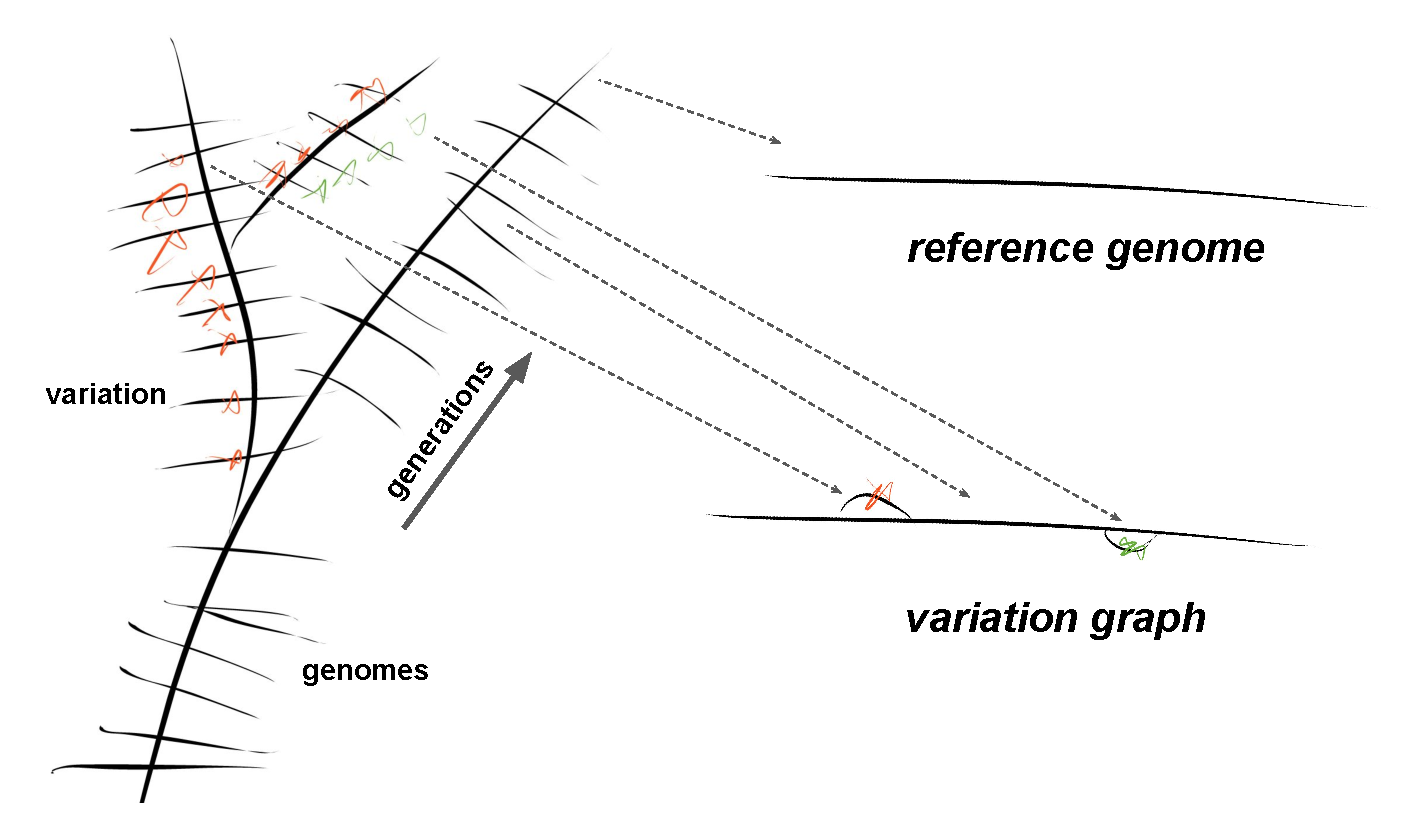
\includegraphics[width=1.0\textwidth]{Chapter1/Figs/phylogeny_and_vg.pdf}
  \caption{
    The tree of life, reference genomes, and variation graphs.
    } 
\label{fig:tree_of_life}.
\end{figure}

Resequencing has arisen in response to the technical properties of the most commonly-used DNA sequencing technologies.
These ``second generation'' sequencing-by-synthesis technologies produce abundant and inexpensive short reads of up to 250 base pairs, and in the past decade have become the largest source of data in the DNA sequencing market.

Higher sequencing costs previously motivated the application of expensive computational approaches to analyze all the sequences of interest simultaneously.
The decades prior to the development of cheap sequencing saw the use of multiple sequence alignment algorithms with high computational complexity.
Analyzing hundreds or thousands of sequences with such techniques is expensive but justifiable given the costs of acquiring them.

However, such approaches became \DIFdelbegin \DIFdel{completely inconceivable }\DIFdelend \DIFaddbegin \DIFadd{too expensive }\DIFaddend as new sequencing technologies allowed the generation of tens and then hundreds of gigabytes of data in a single run.
The new, low-cost techniques allowed joint analyses of thousands of genomes from a single species.
Resequencing provided a practical means to complete these analyses.
\DIFdelbegin \DIFdel{The }\DIFdelend \DIFaddbegin \DIFadd{By relating data to a common linear reference system, the }\DIFaddend alignment phase could be completed independently and in parallel, with each sample compared to the common reference genome\DIFdelbegin \DIFdel{, and only }\DIFdelend \DIFaddbegin \DIFadd{.
Only }\DIFaddend in a final phase of analysis might all the genome data be collected together for the inference of alleles at a given genetic locus.
\DIFdelbegin \DIFdel{By enabling the analysis of genomes at a previously unthinkable scale, resequencing became the core genome inference pattern in genomics.
The standardization of data formats promulgated in large genome sequencing projects supported the separation of different phases of analysis, yielding a rich ecosystem of interacting tools.
}\DIFdelend %DIF > This approach affords scalability to genomic analysis, and has become standard within the field wherever large numbers of samples must be considered.
%DIF > By enabling the analysis of genomes at a previously unthinkable scale, resequencing became the core genome inference pattern in genomics.
%DIF > The standardization of data formats promulgated in large genome sequencing projects supported the separation of different phases of analysis, yielding a rich ecosystem of interacting tools.

In resequencing, the reference sequence shapes the observable space\DIFdelbegin \DIFdel{in a process that is often called }\DIFdelend \DIFaddbegin \DIFadd{, resulting in an effect known as }\DIFaddend \emph{reference bias}.
DNA sequencing reads that contain sequence which is divergent from or not present in the reference sequence are likely to be unmapped or mismapped.
This results in lower coverage for non-reference alleles, in effect forcing new samples to appear more similar to the reference than they actually are.
Divergence itself frustrates the genome inference process, as alignment may produce different descriptions of diverged sequences depending on the relative position of the read.
Alignment works best when the sequences we are aligning are similar to the reference.
Increasing divergence requires greater computational expenditure to overcome reference bias.

We can avoid reference bias by working on pure assemblies generated only from the sequencing data in our experiment and unguided by any prior information.
Doing so can be rigorous, but comes at a significant cost\DIFdelbegin \DIFdel{, especially when the assembly algorithm requires us to load all the sequencing data into memory simultaneously.
We will require much higher coverage to obtain the same level of accuracy in our assembly as we will have when resequencing, and our read lengths will limit the length of contiguous sequences we can infer.
Virtually all assembly algorithms lose information about their source reads through the process of assembly, and this information must be somehow reconstituted if we wish to apply downstream algorithms to the input data in the context of the output of the assembler.
%DIF < No practical algorithm allows us to jointly consider all the samples in a large sequencing experiment in the context of an assembly generated from their reads.
}\DIFdelend \DIFaddbegin \DIFadd{.
Obtaining whole genome }\emph{\DIFadd{de novo}} \DIFadd{assemblies requires greater sequencing and computational costs than resequencing, putting this approach out of reach for many study designs.
}\DIFaddend 

Genome assemblers frequently use a graphical transformation of their inputs that supports algorithm steps used to infer contigs implied by the reads.
These data structures are typically bidirectional graphs in which nodes are labeled by sequences and edges represent observed linkages between sequences.
If constructed from a set of reads that fully cover the genome, it can be shown that such a graph contains the genome which has been sequenced.
In effect, the assembler works to filter the edges from the graph and un-collapse repeats in order to establish a sequence assembly.

In this work I repurpose the assembly graph data model to build a pangenomic reference system.
Assembly graphs are designed to represent the full set of genomic information to which they are applied, so it is natural to use them to develop coherent reference systems for unbiased sequence analysis.
By building a conceptual framework and data structures that enable resequencing against this structure, we can mirror the patterns and workflows that have already been developed for resequencing.
This allows us to retain the benefits of parallel analysis even while we resolve the issue of reference bias.
By recording genomic sequences as paths through this graph I provide anchors for existing annotations and positional systems within the pangenome.
I call these bidirectional sequence graphs with paths \emph{variation graphs}.


\begin{figure}[htbp!]
  \centering
  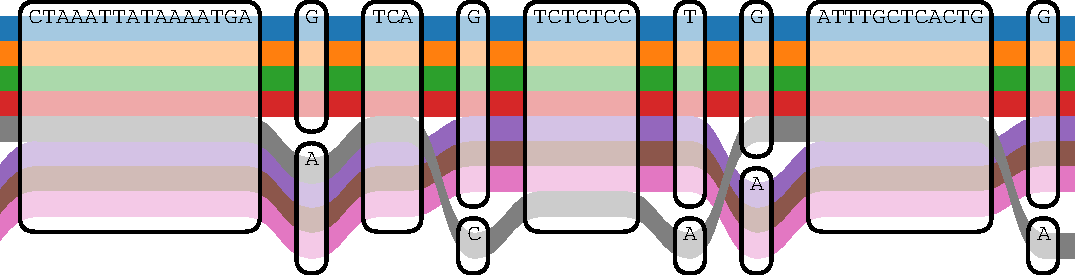
\includegraphics[width=1.0\textwidth]{Chapter1/Figs/vg_tubemap.pdf}
  \caption[A variation graph]{
    A fragment of a variation graph built from fully-assembled \emph{Saccharomyces cerevisiae} genomes.
    Colored paths represent genomes which traverse sequences (nodes).
    Edges are implied by the path structure of the graph.
    The construction and properties of the graph are described in section \ref{sec:yeast_cactus}.
    This visualization was rendered using the SequenceTubeMap \url{https://github.com/vgteam/sequenceTubeMap}.
    } 
\label{fig:variation_graph_tubemap}.
\end{figure}

\DIFdelbegin \DIFdel{In this chapter I will provide background context for my work.
I will cover }\DIFdelend \DIFaddbegin \DIFadd{This chapter provides historical justification for the need for an integrative model for sequence analysis like the variation graph.
I contextualize my work within }\DIFaddend the history of DNA sequencing \DIFdelbegin \DIFdel{methods}\DIFdelend \DIFaddbegin \DIFadd{(\ref{sec:genome_inference})}\DIFaddend , assembly algorithms \DIFdelbegin \DIFdel{, and the development of reference genomes and their use in resequencing.
Finally, I will review similar data models that are used in genome inference.
In the }\DIFdelend \DIFaddbegin \DIFadd{(\ref{sec:genome_assembly}), resequencing methods (\ref{sec:reference_genomes}), and pangenomic models (\ref{sec:pangenomes}).
This deep introduction is meant to justify the need for an integrative model like the variation graph to serve as a coordinating system in a research setting characterized by increasing data scale and complexity.
Readers who need no further introduction to these issues should continue to section \ref{sec:graphical_techinques}, which reviews recent work on algorithms based on data models similar to variation graphs.
}

\DIFadd{The }\DIFaddend remainder of the \DIFdelbegin \DIFdel{work }\DIFdelend \DIFaddbegin \DIFadd{thesis builds on this foundation.
In chapter \ref{chapter:variation_graphs}, }\DIFaddend I describe data structures and algorithms that allow the use of variation graphs as a reference system for unbiased genome inference\DIFdelbegin \DIFdel{, and }\DIFdelend \DIFaddbegin \DIFadd{.
Finally, in chapter \ref{chapter:applications}, I }\DIFaddend demonstrate the benefits of this approach with a series of \DIFdelbegin \DIFdel{experiments}\DIFdelend \DIFaddbegin \DIFadd{experimental case studies}\DIFaddend .

\section{Genome inference}
\DIFaddbegin \label{sec:genome_inference}
\DIFaddend 

% What do we mean by genome inference
% half page
Not two centuries have passed since the first experiments that demonstrated the existence of genetic material \cite{mendel1866versuche}.
In the first part of the twentieth century, these ideas about heredity grew into the core of a modern synthesis linking biological micro- and macro-evolutionary theory to the quantitative basis of genetics \cite{huxley1942evolution}.
It was understood that DNA encoded the information that gave rise to biological structures \cite{avery1944studies}.
The discovery of the structure of DNA in the 1950s \cite{watson1953molecular} made clear the nature of that information and the mechanism for its faithful transmission from generation to generation.
This knowledge, coupled with the sequencing and synthesis of proteins, which demonstrated that they had distinct polymeric chemical identities \cite{sanger1951amino} led to Crick's postulation of the ``central dogma'' of biology \cite{crick1958protein,crick1970central}.
Simply stated, the ``dogma'' argues that in living systems' information is transcribed from DNA to RNA and ultimately translated into proteins, which guide and structure the cell and thus living organisms.
The central dogma clarifies the significance of the sequence of the genome, and over the following decades a series of projects scaled up the throughput and fidelity of DNA sequencing until \emph{genome inference} became a practical and everyday reality in biology.

\subsection{Reading DNA}
% Genome sequencing techniques
% half page

The quest to sequence genomes began with arduous and sometimes dangerously radioactive experimental techniques, in which years of researcher time could be spent in obtaining sequences of tens of bases from partly-characterized sources.
It has then progressed through three distinct phases.
In the first, these early laboratory techniques gave way to automated sequencing using chain terminator chemistry, and related techniques were ultimately used to generate genome sequences for human and a number of organisms, albeit at high costs.
In the second phase, \emph{multiplex} sequencing reactions were used to miniaturize the chain terminator reaction and observe its progression using fluorescent imaging or electrical sensing, evoking a drop in cost per sequenced base of many orders of magnitude, and simplifying library preparation steps dramatically by sequencing clones of individual molecules.
The third wave of development has been characterized by two techniques which allow realtime observation of single DNA molecules.
These produce enormously long read lengths that are limited by the molecular weight of input DNA, but produce readouts with high per-base error rates.
Supporting the second and third wave are methods that allow for haplotype-specific sequencing and the observation of long range structures in the genome.

\subsubsection{The old school}
% Sanger sequencing, BACs, etc.

In the 1970s a group led by Walter Fiers published the first complete gene \cite{jou1972nucleotide}, and then genome sequence \cite{fiers1976complete} from the MS2 bacteriophage using laborious digestion and 2-dimensional gel electrophoresis techniques to sequence RNA based on work by Fredrick Sanger and colleagues \cite{sanger1965two, adams1969nucleotide}.
To avoid the limitations of digestion based assays, Ray Wu and colleagues developed a sequencing technique based on the partial blockage of DNA polymerization with radiolabeled nucleotides \cite{wu1972nucleotide, padmanabhan1974chemical}.
Subsequently, Sanger developed a reliable DNA sequencing method based on the same DNA polymerization chain-termination concept by dividing the sequencing reaction into four, one for each base, and sorting the resulting DNA fragments in parallel on an acrylamide gel \cite{sanger1977dna}.
Optimized and implemented using fluorescent chemistry \cite{strauss1986specific}, this approach, now known as Sanger sequencing, became the foundation of the first commercial sequencing machines in the late 1980s.

Sanger sequencing was the workhorse standard of biology for nearly 30 years, from the late 1970s until the mid 2000s.
Its read length is limited by the reaction efficiency required to obtain a fraction of terminations at every base in the sequence.
In practice, reads of 500 to 1000 base pairs can be obtained.
With clonal DNA as input the per base accuracy of the method is extremely high, as each base readout reflects the termination of large numbers of molecules \cite{castiblanco2013primer}, a feature which has ensured it remains important for validation of sequencing results \cite{sikkema2013targeted}.
However, heterogeneity in the input DNA library can produce muddled signals that rapidly become uninterpretable.
Insertions and deletions (indels) will cause a loss of phase in the sequencing trace \cite{tenney2007tale}, a problem which is still encouraging algorithm development \cite{hill2014poly}.
In order to sequence whole genomes, which are often heterozygous, laboratory techniques were developed to allow the segregation of clonal DNA as a substrate for sequencing.
These include bacterial artificial chromosomes (BACs) and their equivalent in yeast (YACs) \cite{monaco1994yacs}.
The effective read length could be increased by using ``mate pair'' techniques, in which the ends of a longer molecule would be sequenced \cite{schmitt1996framework}.
To yield fully assembled genomes, these data required the development of suitable computational techniques \cite{myers2000whole}.

\subsubsection{``Next generation'' sequencing}

In the late 1990s and early 2000s, several groups began exploring alternative sequencing strategies.
In the ultimately dominant one, DNA that has been clonally arrayed on a surface is directly sequenced using fluorescent imaging.
Sequencing progresses through the synthesis of the second strand of each of the molecules, and so these techniques are typically called ``sequencing-by-synthesis.''
This modality allowed for a massive parallelization of the sequencing reaction, and has resulted in a dramatic reduction of cost.

In 2003 George Church and colleagues demonstrated that individual sequences could be read from polymerase colonies or ``polonies'' suspended in an acrylamide gel using fluorescence microscopy \cite{mitra2003fluorescent}.
This fluorescent imaging model became the basis for ``next generation'' sequencing \cite{shendure2008next}.
Contemporaneously, a sequencing-by-synthesis method which is now known as Illumina dye sequencing, was implemented using laser fluorescent imaging and reversible terminator technology developed by Shankar Balasubramanian and David Klenerman at Solexa (later acquired by Illumina) \cite{balasubramanian2004arrayed, bentley2008accurate}.
Rather than polymerase colonies embedded in an emulsion or gel, Solexa's technology relied on ``bridging PCR'', in which the polymerized clones of a particular fragment were locally hybridized to an adapter-bearing surface of a flowcell.
Controlled synthesis of the second strand, based on reversible terminator chemistry \cite{canard1994dna} and fluorescently labeled dNTPs, is then used to observe the sequence of the DNA molecule in each colony.

A diverse set of similar approaches were explored during this period, although few saw more than limited success in the sequencing market.
Church's group focused on a hybridization based sequencing protocol proceeded by an emulsion based polony PCR step \cite{shendure2005accurate}, and later attempted to commercialize an open source sequencing device (the Polonator)\footnote{My interest in open source projects, developed while an undergraduate studying the social sciences, led me to work on this device. The project introduced me to biology, bioinformatics, and DNA sequencing, which have attracted my interest and effort ever since.}.
In ion semiconductor sequencing direct observation of pH changes were used to determine DNA sequences \cite{rusk2010torrents}.
454 Life Sciences' ``pyrosequencing'' implementation used a luciferase reporter assay to track the progression of DNA synthesis \cite{margulies2005genome}, and it was used to generate the first whole genome human sequence using ``next generation'' techniques \cite{wheeler2008complete}.
Helicos commercialized the first single-molecule sequencing system, using a similar chemistry to Illumina's but observing single molecules rather than pools, which proved technically challenging and only saw use in its own development \cite{harris2008single}.

Illumina's sequencing protocol provides greater throughput and a superior error profile relative to these methods.
Its low per base error rates and handful of context specific error types simplify analysis \cite{allhoff2013discovering}.
It is unsurprising that the vast majority of sequencing data produced in the 2010s comes from Illumina sequencers.
Illumina's sequencing technology is characterized by short reads (<250bp) with per-base accuracy ($\approx 99.5\%$) comparable to that of Sanger sequencing.
Although the read length has been increased by optimization of the technology, the difficulty of achieving perfect per-base reaction efficiency apparently prevents greater extension of the read length.

A number of methods extend the genome inference capacity of Illumina sequencing, allowing it to be used to infer long haplotypes and genome organization.
Moleculo, and later 10X Genomics commercialized barcode-guided haplotype sequencing and assembly \cite{zheng2016haplotyping}.
The later has focused on providing raw tag information that could be used downstream by an array of haplotype-resolution and assembly tools \cite{mostovoy2016hybrid}.
The single template aspect of Illumina paired end sequencing allows longer contiguous DNA reads to be obtained by merging partly-overlapping read pairs computationally \cite{magovc2011flash}.
Single-cell DNA template strand sequencing (strand-seq) can be used to obtain reads from only one half of the chromatids in a single cell \cite{falconer2012dna} via bromodeoxyuridine (BrdU) treatment and cleavage of the nascent strand, which can aid in haplotype reconstruction \cite{porubsky2016direct}.
The Hi-C method \cite{lieberman2009comprehensive} uses bisulfite treatment to generate read pairs that are likely to physically co-locate \emph{in vivo}, thus enabling the mapping of long range DNA and chromatin interactions.
It may be combined with other sequencing information to obtain estimates of the syntenic ordering of contigs produced by assembly \cite{ghurye2018integrating}, which has already been used to obtain \emph{de novo} reference quality genomes in several difficult sequencing projects including amaranth \cite{lightfoot2017single}, \emph{Aedes aegypti} \cite{dudchenko2017novo}, and the domestic goat \cite{bickhart2017single}.

\subsubsection{Single molecules}

All previously described sequencing techniques are dependent on the observation of pools of molecules.
These methods benefit from amplification of DNA, which increases signal, but also adds and a potential source of error to DNA sequencing.
They also suffer from de-phasing resulting from imperfect stepwise reaction efficiency, which fundamentally limit the maximum length of an accurate read.
A method to sequence single molecules accurately would theoretically allow longer read lengths, but this requires the difficult, direct observation of DNA.
Efforts to develop such a method have been continuously underway throughout 2000s and 2010s.
Two successful commercial sequencing platforms based on this principle are rapidly defining a new technical phase of genome inference.

By utilizing zero-mode waveguides (ZMWs) to observe DNA polymerase in real time, Pacific Biosciences (PacBio) generated the first successful commercial single-molecule sequencing system \cite{eid2009real}.
In this platform, DNA polymerase is immobilized in sub-diffraction size, picoliter detection volumes at the bottom of wells formed in aluminum on a glass slide \cite{korlach2008selective}.
Single stranded DNA and fluorescently-labeled dNTPs are added to the buffer above the ZMWs.
As synthesis progresses, the fluorophore attached to the DNA base that is being incorporated will tend to remain inside the ZMW longer than would be expected due to random diffusion of the dNTPs, allowing a readout of the sequence of incorporated bases as a series of fluorescent pulses.
The base-level error rate of sequencing is high, up to 15\%.
It is difficult to perfectly observe the series of fluorophores pulled into the well, and random occupancy is often indistinguishable from polymerization-mediated occupancy, which results in insertion errors.
Although subtle context dependent biases do exist \cite{ono2012pbsim}, due to their genesis in Brownian motion, the errors themselves may be considered as almost perfectly random in analysis \cite{ross2013characterizing,myers2014efficient}.
In recent years PacBio's system has become a foundational technology in genome sequencing, with many recent genome assemblies completed using it \cite{rhoads2015pacbio}.

The idea that electrophoresis of DNA through nanometer scale pores might allow the direct sequencing of DNA was first postulated in the late 1980s by David Deamer and others \cite{deamer2016three}.
While the sequencing model itself is among the simplest ever proposed, it would take twenty-five years of work \cite{kasianowicz1996characterization,purnell2008nucleotide} before the technique was brought to market by Oxford Nanopore (ONT) \cite{mikheyev2014first} and used to fully sequence genomes \cite{loman2015complete, jain2018nanopore}.
In this approach, a DNA strand is pulled through a nanometer pore by electrophoresis.
The specific DNA bases in the pore effect characteristic changes in the electric current density, and the DNA molecule can be read by measuring the changes in current over time.
Due to context and history-dependent effects that distort the signal, the measured patterns in the current flux must be interpreted by sophisticated models that have been trained to convert the traces to DNA sequences \cite{david2016nanocall}.
As with PacBio, its per-base error rate approaches 15\%.
In practice nanopore sequencing has the highest error rate of any commercially available method, which reflects the difficulty of mapping between the observed signal and the underlying DNA sequence.
Nanopore sequencing can also obtain the longest reads of any sequencing technology, with megabase-scale reads reported by some users.

%, single molecule ONT/PacBio (3rd gen)

\subsection{Genome assembly}
\label{sec:genome_assembly}

Due to technical limits that are unlikely to ever be fully eliminated, individual DNA sequence reads are rarely able to cover the entire genome of an organism.
This means that in many cases, the best sequencing data possible is a set of random reads sampled from fragments of the genome. 
In whole genome ``shotgun'' sequencing the genome is fragmented, perhaps by sonication or enzymatic digestion, and the resulting fragments are sequenced and then reassembled using computer programs \cite{gardner1981complete, sanger1982nucleotide}.
This process necessitates a reconstructive step in which the information obtained from the sequenced fragments is reassembled into the whole genome from which they arose.
This process is known as \emph{assembly}, and computer algorithms implementing it have been used when inferring genome sequences since the generation of the first whole genome sequence for bacteriophage $\varphi$X174 in 1977 \cite{sanger1977nucleotide, staden1979strategy}.

The earliest assembly algorithms have come to be known as ``overlap-layout-consensus'' (OLC) algorithms, due to their three-phase strategy.
They first establish a set of head to tail overlaps between reads (overlap), an $\approx O(N^{2})$ order problem when all pairwise relationships are considered between $N$ sequence reads.
However, given an efficient method to find read pairs that are very likely to match together, the overlap step remains tractable as the overall complexity of matching can be reduced to be approximately quadratic in read depth and linear in genome size \cite{huang1992contig}.
These overlaps are then used to establish an estimate of the ordering of the reads (layout).
The layout is then used to generate a consensus sequence through heuristics or dynamic programming over the layout \cite{kececioglu1995combinatorial}.
This final phase is equivalent to the multiple sequence alignment (MSA) problem, although instead of generating an MSA as output methods would typically take the consensus sequence, as the objective is often to reconstruct a linear representation of the input genome.
Early assemblers committed frequent assembly errors, which necessitated time-consuming manual ``finishing'' \cite{gordon1998consed}.
The OLC assembly approach was utilized by genome projects for the following twenty-five years, including in the public Human Genome Project (HGP), where BAC clones of 150kb fragments of the genome were sequenced, initially assembled by algorithm and finally manually finished into the ``golden path'' that would become the reference genome \cite{international2001initial}.

In principle, the assembly process could be fully automated, but as late as the early 1990s this frequently was not seen as feasible due to the lack of reliable algorithms \cite{mahy1991sequencing}.
The improvement of OLC algorithms eventually met the challenge, yielding methods such as PHRAP \cite{green1999phrap} (a quality aware assembler that saw extensive use downstream of Sanger sequencers), TIGR \cite{sutton1995tigr} (which was used in the generation of the first assembly of a free living organism, the 1.8Mbp genome of \emph{Haemophilus influenzae} \cite{fleischmann1995whole}), GigAssembler \cite{kent2001assembly} (which was used by the HGP), and the Celera assembler \cite{myers2000whole,miller2008aggressive} (which saw extensive use in the generation of early large whole genome assemblies in the late 1990s and early 2000s, including the privately funded genome project \cite{venter2001sequence}\footnote{This project apparently still relied on data produced by the HGP \cite{waterston2002sequencing}, but the significance of this reliance was disputed by researchers involved in the private project \cite{myers2002sequencing}, who argued that the manner in which they used the public sequences avoided contamination by manual finishing done by the HGP.}.)
The process implemented in the Celera assembler (including repeat masking) has remained essential to the genome assembly problem until the present.

In 2005, Myers formalized an idealized version of the assembly problem in the \emph{string graph} data structure \cite{myers2005fragment}, which is a sequence graph induced from the overlaps in a set of shotgun sequencing reads.
This model demonstrates that repeats greater than the length of a sequence read will collapse into single copies in the graph, while unique sequences will form loops between different repeat classes that flank them.
The string graph can be shown to represent the full information available in the input sequence data, and successful assembly algorithms are built around an induction of the string graph via the construction of the FM-index \cite{ferragina2001experimental} from Illumina read sets \cite{simpson2010,simpson2012efficient,li2015fermikit}.
If not using compressed data structures and low-error reads, the repeats are often irresolvable and may be masked from the assembly process to improve performance on the tractable non-repetitive regions of the genome, which is a strategy still promoted and employed by Myers \cite{myers2014efficient}.
Canu and FALCON, which to some extent stand as contemporary implementations of the Celera assembly process, are among the best-performing assemblers for noisy single-molecule sequencing data that is the mainstay of current genome assembly projects \cite{chin2016phased,koren2017canu}.
These and similar methods have shown that long reads can be used to fully assemble genomes without human finishing \cite{loman2015complete,jain2018nanopore}.

The repeat problem has been tackled in various ways, but one of the most enduring solutions resolves the issue through the reduction of the assembly overlap graph to a de Bruijn graph (DBG) \cite{pevzner2001eulerian}.
In this approach, the read set is fragmented into all subsequences of reads of a given length $k$, and a graph is constructed where $k$-mers label nodes and overlaps of $k-1$ between successive $k$-mers induce edges representing linkages between them.
The de Bruijn graph simplifies the representation of the read set, providing a clean basis for assembly algorithms.
It enabled the first \cite{zerbino2008velvet,simpson2009abyss,iqbal2012novo}, and most memory-efficient assembly methods for short read sequencing data, with techniques like bloom filters \cite{chikhi2013space}, succinct DBGs \cite{bowe2012succinct,li2015megahit}, and minimizer partitioning \cite{chikhi2016compacting} applied to generate a compressed representation of the graph.
DBG based assemblies suffer from the loss of information induced through the $k$-merization of their input, causing a reduction in assembly contiguity \cite{earl2011assemblathon}, although in practice this can be mitigated by reconsideration of the input reads and read pairs \cite{butler2008allpaths}.
They also are applicable only where the sequence error rate is low enough for overlapping reads to be expected to have exact matching $k$-mers of the appropriate size (typically, $k \in [20 \ldots 50]$ base pairs), and as such cannot be applied to third generation single molecule sequencing due to its inherently high error rate.

Many of the sequencing methods I have described above are still in use today.
Each popular method, as it fades from use, remains relevant in a niche area where its particular properties provide it a comparative advantage.
As a result, we are not presented today with a single ideal sequencing method, but a menagerie of approaches, each with its own limitations and benefits, and current assembly pipelines require thoughtful design to incorporate these myriad sources of information.
It would appear that in order to use these many technologies to generate the best-possible assemblies we must bring them together in a single model \cite{chaisson2018multi}.
A current development in assembly focuses on the design of a common interchange format for which to organize such assembly processes, which has been implemented as the GFA v1 and v2 formats.\footnote{\url{https://github.com/GFA-spec/GFA-spec}}
This file format and the data model it implies is an essential link between the work that I present later in this thesis and the problem of genome inference.

\section{Reference genomes}
\DIFaddbegin \label{sec:reference_genomes}
\DIFaddend 

Obtaining a single genome sequence \emph{de novo} is an arduous task, and remains a complex problem.
The result is a valuable object which can be used to lower the cost of subsequent analyses and enable direct whole genome comparisons which provide a full perspective on the genetic relationship between multiple individuals or species.
The need for reference genomes is clear, and they are collected in open public databases to allow their dissemination and use by researchers.
NCBI's RefSeq release 89 of July 13, 2018 contains some 81,345 organisms\footnote{\url{https://www.ncbi.nlm.nih.gov/refseq/}}, although it should be noted that only a small fraction of these genomes are eukaryotic.
Recent developments in long read, single molecule sequencing have enabled great decreases in the cost and complexity of generating high-quality genome assemblies, supporting a recent project to generate reference quality genomes of ten thousand vertebrates \cite{genome2009genome,koepfli2015genome}.

The reference genome serves as an anchor for annotations that describe sequences and regions of interest within the genome, such as genes, exons, chromatin structures, DNA interacting proteins, and genetic variation \cite{sherry2001dbsnp,quinlan2010bedtools,encode2012integrated}.
An established reference genome can serve as a conceptual foundation for the communication and interpretation of scientific results \cite{kent2002human}, and is seen as essential for collaboration and the development of a genome research community in a particular organism \cite{smith1998functional,cherry1998sgd}.

Reference genomes tend to represent only a single version of each genomic locus.
This conceptual simplicity is a core feature of their public use.
Although the issue of genetic diversity has always been appreciated by those who work with genomes, expediency has encouraged the use of linear models for reference genomes.
Within the HGP, members of the consortium could observe diversity within the BAC clones that they had sequenced from different human donors, and initiated a debate about the inclusion of heterozygosity in the reference itself.
Ultimately, a graphical model was seen as too complicated, and practicality necessitated the publication of a linear reference based around what came to be called the ``golden path'' through the assembly\footnote{Personal communication with David Haussler.}.
Since early releases, the human reference genome has included alternative versions of some regions, with current releases including alternates for around 200 loci \cite{schneider2017evaluation,church2018genomes}, but these are represented as linear sequences without a unifying alignment between them, which complicates their use in resequencing and annotation \cite{jager2016alternate}.

% history of reference sequences
% use of the reference sequence in analysis
\subsection{Resequencing}
\DIFaddbegin \label{sec:resequencing}
\DIFaddend 

Due to the high cost of obtaining error-free, full length genomes, standard practice will use the best genome assembly for a given organism as a \emph{reference genome} when analyzing the sequences of other organisms from the same species.
To do so, the genomes of the other individuals do not need to be fully assembled, and instead shotgun sequencing libraries from these new individuals may be aligned back to the reference to find small differences between the genomes.
To distinguish it from whole genome sequencing and assembly, this process is known as \emph{re}sequencing.

Resequencing has two phases.
In the first phase, reads from the sample or samples under study are aligned against an appropriate, genetically similar, reference genome.
In the second phase, the aligned reads (alignments) are processed together locus by locus to determine allelic variation within the samples relative to the reference genome.

\subsection{Sequence alignment}
\label{sec:sequence_alignment}

An \emph{alignment} expresses one sequence in terms of a set of positions, edits, and matches to another.
Algorithms to determine the most plausible alignment between a pair of sequences have as long a history as sequencing itself.
The first significant attempts to algorithmically assess sequence homology and divergence between protein sequences arose in the 1960s with Fitch's method for homology detection \cite{fitch1966improved}.
To account for insertions and deletions, this method required the comparison of many subsequences of two sequences to be compared, resulting in poor computational bounds.
In 1970, Needleman and Wunsch responded with an O(NM) time algorithm for the global alignment of sequences \cite{needleman1970general}.
Given strings to compare of length $N$ and $M$, the algorithm builds an $M \times N$ matrix in which any possible full length alignment between both sequences can be expressed as a path through a series of cells.
The matrix is designed such that a match corresponds to the shortest (diagonal) path through the matrix, and insertions and deletions correspond to horizontal or vertical movements.
To determine the most-likely path, Needleman and Wunsch apply a recurrence relation dependent on the characters at each pair of positions in the strings and the values of the cells above and/or to the left.
This implements a dynamic programming (DP) method \cite{bellman1952theory}.
For each cell, the score is given as the maximum of: the score of cell to the diagonal plus a bonus if the corresponding sequence characters are the same and minus a penalty if they are different; and the scores of the cells above and below minus a penalty corresponding to the weight given to an insertion or deletion.
Finally, we determine the optimal path beginning from the opposite extreme cell of the matrix from where the scoring began, in which we walk back through the successive maximum scores until reaching the opposite extreme corner of the matrix.
This ``traceback'' encodes the alignment, which is most-simply represented as a vector of pairs of matched bases in each sequence.
It can be shown that provided full evaluation of the dynamic programming problem, the optimal alignment is obtained given a set of scores parameterizing the recurrence relation.

This alignment algorithm is known as a ``global'' alignment algorithm, in that the alignment covers all bases of both sequences.
In practice, this type of comparison is not always needed, and it can be advantageous to obtain only the optimal sub alignments between sequences.
Smith and Waterman provided a clean modification of the algorithm of Needleman and Wunsch, altering it to prevent negative scores, which allowed it to produce optimal ``local'' alignments \cite{smith1981comparison}, while ignoring regions unlikely to contain significant homology.
The algorithm, further refined by Gotoh \cite{gotoh1982improved} to enable affine gaps\footnote{In affine gap schemes the cost of a gap per base decreases as its length increases. Such a scheme approximates the $\zeta$-distributed excursions of a particle under Brownian motion, which structure the length of insertions and deletion mutations observed in nature.} and computation in $O(MN)$ time, is today one of the most important in genome analysis.
The amount of work on this topic is considerable, and the subsequent decade yielded numerous modifications of the basic alignment concept, for instance reducing the memory bounds to $O(N)$ through a divide and conquer approach \cite{myers1988optimal}, and further explorations of affine gap scoring schemes \cite{altschul1986optimal,gotoh1990optimal}.
Subsequent works have offered improved implementations, using vectorized instructions to improve the runtime of the algorithm \cite{farrar2007striped} and heuristics to selectively evaluate only part of the DP matrix \cite{suzuki2017acceleration}.
However, such changes were not sufficient to enable alignment against large sequence databases.

$O(MN)$ algorithms for sequence alignment are impractical when either $M$ or $N$ becomes large.
Naturally, as sequence databases grew and the size of sequenced genomes increased, heuristic strategies to efficiently reduce the alignment problem size were introduced.
When aligning a short sequence against a large database we expect to obtain a sensitive alignment, but provided sufficient homology between the sequence and the database it is unlikely that we need to evaluate the full problem using an algorithm like Smith-Waterman-Gotoh (SWG).
By indexing either the query or target set of sequences to efficiently obtain patterns of exact matches, candidate sub-regions of both can be isolated and submitted for more sensitive alignment.

This strategy was implemented in the mid- to late-1980s in the FASTA \cite{pearson1988improved} and BLAST \cite{altschul1990basic} alignment algorithms.
FASTA first uses a seeding step that finds exact matches between the query and target, using chains of short $k$-mer seeds to establish the longest matching subsequences.
A few of the best scoring candidates are enumerated and evaluated using a banded SWG algorithm.
In contrast, BLAST implements a fully heuristic alignment process based solely on the $k$-mer seeds and ungapped alignment.
This is much faster than FASTA but can perform slightly worse with highly divergent sequences.
BLAST's heuristic alignment is many orders of magnitude faster than full DP based algorithms at a minor cost to accuracy.
The popularity of BLAST in biology\footnote{The BLAST1 paper has been cited more than 70,000 times as of August 2018.} is clear evidence of the importance of the alignment problem to all kinds of genomic analysis.
It is also evidence that minor losses in accuracy are acceptable given the cost of sequence analysis in large data sets.
Jim Kent's Blast-like alignment tool (BLAT) indexes the target set with non-overlapping $k$-mers and queries all $k$-mers in the reads, yielding a method that is less sensitive but several orders of magnitude faster again than BLAST \cite{kent2002blat}.

As reliable commercial second-generation sequencing systems became available the rate of sequence data acquisition growth rapidly outstripped the rate of improvement in computing performance \cite{leinonen2010sequence,kodama2011sequence}.
This necessitated further improvements in the computational cost of sequence alignment.
The most-widely used of these methods focused on the increasingly prevalent problem of aligning short reads to reference genome type sequence databases.
Due to the high quality of the reference sequence, low error rate of the short ($\leq$100bp) reads, and low nucleotide diversity of humans (where $\theta \approx 10^{-3}$), algorithms that focused on exact string matching had great success.
Much like BLAST and BLAT, the first wave of aligners capable of indexing the human reference genome and aligning short reads to it utilized exact $k$-mer matching via hash tables followed by local alignment \cite{li2008soap,lee2014mosaik,li2008mapping}.
Substantial improvements would be yielded by the development of aligners based on contemporary developments in compressed data structures.

\DIFaddbegin \subsubsection{\DIFadd{Compressed full text indexes}}
\label{sec:compressed_full_text_indexes}

\DIFaddend The suffix tree \cite{weiner1973linear} encodes all suffixes of a sequence $S$ in the structure of a tree such that the suffixes may be enumerated by a depth first search (DFS) of the tree.
This structure can be used to determine if a given sequence $q = c_{1}c_{2}\ldots c_{|q|}$ is present in $S$ in $O(|q|)$ time.
Search begins at the root, progressing across the topology (edge or node) of the tree which is labeled with the next character until no further matches may be found.
By labeling the tree with the sequence positions corresponding to each node, the search may also yield the positions of the exact matches detected within $S$.
Suffix trees may be built in linear time and space relative to their input \cite{ukkonen1995line}, and support diverse algorithms for string comparison \cite{apostolico1985myriad}, such as whole genome alignment \cite{delcher1999alignment}, but they require relatively large amounts of memory per input base.
They were superseded by equivalent data structures with better memory bounds such as the suffix array\DIFdelbegin \DIFdel{(}\DIFdelend \DIFaddbegin \DIFadd{, }\DIFaddend which represents the \DIFdelbegin \DIFdel{tree in a linear array of suffix sort ranks) }\DIFdelend \DIFaddbegin \DIFadd{lexicographically ordered suffixes as a vector of numbers }\DIFaddend \cite{manber1993suffix}, and its compressible sibling the Burrows-Wheeler Transform (BWT) \cite{burrows1994block}.
\DIFdelbegin %DIFDELCMD < 

%DIFDELCMD < %%%
\DIFdel{By augmenting the BWT to enable the exact matching via emulation of the suffix tree, Paolo Ferragina and Giovanni Manzini developed the FM-index \mbox{%DIFAUXCMD
\cite{ferragina2000opportunistic,ferragina2004alphabet}}\hspace{0pt}%DIFAUXCMD
.
Given a string $S$, }\DIFdelend \DIFaddbegin \DIFadd{Compressed suffix arrays (CSA) (equivalently, }\DIFaddend the \DIFaddbegin \DIFadd{``fast, minute'' }\DIFaddend FM-index\DIFdelbegin \DIFdel{may be built using a series of transformations and auxiliary data structures that induce the suffix tree by constructing the BWT.
First, we add marker characters for the start and end with lexicographic order less and greater than the rest of the characters in the alphabet, e.g. $\#S\$$.
Conceptually, we take all rotations of the sequence and sort them, yielding matrix $M$, which is sometimes called the Burrows-Wheeler Matrix (BWM), but in fact this is done in a space-efficient manner without the enumeration of the rotations.
This sort has many similarities to the suffix tree, and for instance it can be seen that a lexicographically-ordered DFS through the suffix tree would enumerate the prefixes of the rotations of the sequence preceding the terminal character $\#$ in the same order as they are sorted.
The suffix array $SA$ is given by the vector of the suffix ranks in the sorted order they occur in $M$, and is related to the ordering of characters in the first column $F$, while the BWT is given as the last column, $L$.
If the input text has repetitive patterns, then these will tend to result in runs in the BWT that may be compressed using various schemes.
To emulate traversal of the suffix tree, it is sufficient to construct a function $LF(i)$ which maps between indexes $L[i] = F[j]$ which represent the same character.
This is done by the augmentation of the data structure with array $C$ such that $C[c]$ returns the number of characters in the text that are lexicographically smaller than $c$, and a function $rank(c,k)$ that yields the number of instances of $c$ in the prefix $L[1 \ldots k]$.
Now, $LF(i)$ may be defined as $C[L[i]] + rank(L[i], i)$.
By allowing the traversal of equivalencies between the suffix array and the BWT, $LF$ mapping enables ``backward search''.
Because rotations of $S$ have been ordered in $M$, a given pattern will occur as the prefix of a particular contiguous range of $M$.
We can find all occurrences of a given pattern by maintaining a range }\DIFdelend \DIFaddbegin \DIFadd{) are data structures which combine a compressed representation of the BWT with auxiliary data structures that support rank and select operations on it \mbox{%DIFAUXCMD
\cite{ferragina2000opportunistic,ferragina2004alphabet,grossi2005compressed}}\hspace{0pt}%DIFAUXCMD
.
To support suffix array operations in this compressed context, including pattern matching and positional queries, standard implementations include additional auxiliary information, in particular a sampled subset of the entries }\DIFaddend in the suffix array\DIFdelbegin \DIFdel{within which a given pattern occurs, beginning at $s$ and ending at $e$, which we initially set as $s=0$ and $e=|L|-1$.
To search for a pattern, we obtain $s' = C[c] + rank(s,c) + 1$ and $e' = C[c] + rank(e,c)$, walking backwards through the characters $c$ in our query $q$.
Our search terminates when we complete our query or $e' - s' \leq 0$, which indicates that the previous step in the search did not match our target $S$.
The various matches of $q$ in $S$ may now be obtained by the positions in $SA[s \ldots e]$.
The addition of the longest common prefix (LCP) array on the sorted suffixes can be used to emulate all algorithms on suffix trees in this context \mbox{%DIFAUXCMD
\cite{abouelhoda2004replacing}}\hspace{0pt}%DIFAUXCMD
, and in turn this enables $O(|q|)$ search of queries against $S$.
Of particular relevance to this work, when completing a phase of backward search we could use the LCP to traverse the suffix links in the suffix tree and continue with the next (partially overlapping) maximal exact match}\DIFdelend \DIFaddbegin \DIFadd{.
See section \ref{sec:fmidx_csa} for a detailed review of the important features of these data structures as they relate to string matching}\DIFaddend .

The FM-index is used in modern short-read aligners such as BWA \cite{li2009fast} and BOWTIE \cite{langmead2009ultrafast}, which \DIFdelbegin \DIFdel{used backtracking LF alignment }\DIFdelend \DIFaddbegin \DIFadd{apply a backtracking search algorithm }\DIFaddend to directly align sequences to the suffix array encoded in the FM-index.
This \DIFdelbegin \DIFdel{backtracking search }\DIFdelend \DIFaddbegin \DIFadd{approach }\DIFaddend is fast, but has problems detecting indels (as these require exponentially more backtracks to infer) and performs less well with increasing read length.
In response, the authors merged initial exact matching with a final DP step to yield ``long read'' capable aligners like BWA-SW \cite{li2010fast} and BOWTIE2 \cite{langmead2012fast}.
Further refinements of this concept yielded BWA MEM \cite{li2013aligning}, which uses a heuristic algorithm to determine ``supermaximal exact matches'' (SMEMs) and reseed ``sub matches'' within them using a bidirectional FM-index (the FMD index).
Due to its relative robustness to error and variation, the MEM concept has ultimately prevailed and as of the time of this writing BWA MEM can be seen as the industry standard method for aligning short reads to the genome.

Much of the second generation sequencing data has been generated for humans in medically-motivated genome wide association studies \cite{uk10k2015uk10k} or population survey projects like the 1000 Genomes Project (1000GP) \cite{1000Gphase1,1000g2015}. % TODO not sure about this phrasing
The development of these methods was accelerated by an open, competitive spirit fostered during the 1000GP, whose primary sequencing data remains the largest completely publicly available data set, with more than 100TB of sequence data available for download from public URLs without any authentication.
There, project participants formalized the resequencing process by generating a series of data formats linking the various stages of analysis, including the sequence alignment/map format (SAM) and its binary equivalent (BAM) \cite{li2009sequence} that is the standard output format for contemporary aligners.


\subsection{Variant calling}

DNA sequencing reads of all types contain errors, and genomes contain diversity.
To resolve these errors and infer the genome's state, we aggregate information from many reads mapping to each locus.
In the context of resequencing, this process is known as \emph{variant calling}.
The simplest methods resemble the consensus step in OLC assembly, and are implemented as heuristic filters on the mutually gapped alignment matrix of a set of homologous sequence reads \cite{koboldt2009varscan}.
A Bayesian model can incorporate prior expectations about the genomic state with the available data to generate a posterior estimate of the probability of polymorphism that can propagate uncertainty to downstream analyses.
It can use first principles to integrate various sources of information in addition to the sequence of the reads themselves, including the base quality (BQ), or machine-estimated probability of an erroneous base call, and mapping quality (MQ), which represents the aligner's estimate that the given alignment is a mismapping or ambiguous \cite{li2011statistical}.
A Bayesian approach also supports the joint analysis of many individuals from the same population.
For instance, in a panmictic population under neutral selection the pattern of observed genotypes should be consistent with Hardy-Weinberg Equilibrium (HWE), and to have confidence in a given genotyping call, the evidence for variation should be stronger than the prior odds of there being no genetic variation at the site.

The earliest implementations of Bayesian variant calling and genotyping were applied to expressed sequence transcripts (ESTs) \cite{marth1999general}.
Competition fostered by the 1000GP encouraged the development of variant calling algorithms based on a variety of principles.
The simplest methods would detect variation given pointwise SNP and indel descriptions directly from the alignments \cite{li2009sequence,depristo2011framework}.
However, this technique was shown to be susceptible to inconsistencies in the alignment process, and several groups developed methods that would reevaluate the alignments in a reference-independent manner in order to homogenize the representation of small variation.
These techniques became known as ``local assembly'' variant detection algorithms, and include the windowed haplotype detection implemented in freebayes \cite{garrison2012haplotype} as well as full local \emph{de novo} assembly based on de Bruijn graphs as implemented in Dindel \cite{albers2010dindel}, Platypus \cite{rimmer2014integrating} and the GATK's HaplotypeCaller.
In parallel, several whole genome \emph{de novo} assembly methods, including SGA and Cortex, were applied to the full data set, yielding variant calls that minimized bias towards the reference genome.
The final project results were merged into a population genome assembly using statistical phasing algorithms \cite{browning2007,howie2011,delaneau2012} guided by genotyping results from sequencing and genotyping arrays \cite{1000g2015}.
Members of the 1000GP also developed a file format for describing collections of resequenced genomes, including their genotypes and inferred haplotypes, the variant call format (VCF) \cite{danecek2011variant}, which has become the standard interchange format for sequencing-based variant and genotyping information.

Due to the absence of a reliable truth set, early variant calling method implemented conceptually-derived inference methods rather than machine learning techniques.
Subsequently, projects at Illumina (Platinum genomes) and NIST (Genome in a Bottle) have generated ``truth sets'' for variant calls matched to cell lines for which large amounts of sequencing data is publicly-available \cite{eberle2013platinum,zook2014integrating}.
These truth sets have then enabled the development of ``universal'' variant callers using machine learning techniques \cite{poplin2017creating}\footnote{Along with Nicol\'{a}s Della Penna, I developed a similar but much simpler method based on a linear learner: \url{https://github.com/ekg/hhga}}.
It may be expected that this trend will continue as the number of highly accurate independently sequenced genomes increases.

\subsection{The reference bias problem}

Short reads are insufficient to generate \emph{de novo} assemblies of reference quality, and this issue is exacerbated when they are used in resequencing, as the prior information provided by the reference is relatively strong and can distort our results \cite{sudmant2015integrated}.
Most aligners operate on the principle of matching each sequence read to the linear reference, and differences between the read and the reference induced by both error and variation will tend to reduce the success of mapping.
As I will demonstrate later in this work, reference bias is most severe for larger variants.
However, the bias towards the reference is relevant even for SNPs, a fact which adds great complexity to experimental contexts that are sensitive to slight changes in allele observation count, such as allele specific expression (ASE) quantification from RNA sequencing \cite{stevenson2013sources}, or in the context of short and high error reads as are common in the sequencing of ancient DNA \cite{zhou2017antcaller}.

Advances in sequencing technology can reduce reference bias in some contexts where long reads can be obtained.
Long reads can overlap structural variants that would contain shorter reads, allowing their direct discovery by alignment.
However, costs of second generation sequencing continue to drop, so it seems likely that there will continue to be a cost advantage to resequencing with short reads for the near future.
Nonetheless, reference bias remains relevant even in a future in which all sequencing is completed with long, low-error reads.
As long as the reference is used as a basis space for analysis, it will be impossible to develop unbiased representations of all sequences in a given cohort.
We cannot consistently describe variation in sequences which are not in the reference unless we bring these sequences into communication with each other.
It is non-trivial to establish if structural variants independently described against the reference represent the same allele \cite{chaisson2018multi}.
We can use improvements in assembly methods, such as the linked DBG \cite{turner2018integrating}, to build space-efficient joint assemblies of populations of genomes.
But these approaches are unlikely to improve in efficiency by the many orders of magnitude required to consider applying them directly to sequencing from hundreds of thousands or millions of genomes.

%By laying out the history of the field in detail, I hope to have built a case that such a change is justified and likely to be useful in any likely future state of sequencing and genome inference.
%We have seen that no sequencing method is perfect, and techniques retain utility for long periods of time due to the numerous tradeoffs inherent in all sequencing methods.

%Using two passes over the data, we can allow full communication between all DNA sequences without 

% it is necessarily harder to see things when the become more divergent
% literature review of examples

\section{Pangenomes}
\label{sec:pangenomes}

Following the completion of the 1000GP, researchers have sought to use the population reference established by that project as an input to genome inference processes.
Rather than establishing a single linear reference genome, these methods base their analysis on a representation that contains some or all of the known variation in the species of interest.
In these approaches, the reference system becomes a \emph{pangenome}\footnote{``pan-'' from Greek $\pi\alpha\nu-$, meaning ``all'' or ``every''}, or data space representing all the genomes and their interrelationships.
The term was first used to describe the sequence information obtained from DNA and RNA for a cancer sample \cite{sigaux2000cancer}, but later became an important concept in microbiology as results from bacterial genome sequencing indicated extensive diversity between bacterial genomes \cite{tettelin2005genome,medini2005microbial}.
Due to horizontal gene transfer (driven in large part by the permissive sex lives of bacteria), mobile DNA in the form of viruses and transposable elements, and their enormous population sizes, the genome diversity of many prokaryotes is much greater than that seen in larger, complex organisms.
In microbial pangenomic theory, the main object of interest is the open reading frame (ORF) and its distribution across species in a clade \cite{vernikos2015ten}, with particular interest to classification of ORFs or genes into a gradient between those that are essential and found in every species (the ``core'' pangenome) to those that are found infrequently (the ``dispensable'' pangenome).
The term ``pangenome'' is by no means microbiology-specific, and has also seen use in species contexts where small, homozygous genomes support practical direct whole genome comparison, such as \emph{Arabidopsis thaliana} \cite{cao2011whole}.
With reducing sequencing costs, the levels of diversity in eukaryotic genomes can be more easily appreciated, and in the 2010s evidence has rapidly accumulated that significant levels of large-scale variation occur in the genomes of many species, humans \cite{li2010building,sudmant2010,sudmant2015integrated,chaisson2018multi}, arabidopsis \cite{alonso2016arabidopsis}, brewer's yeast \cite{yue2017contrasting}, and the fruit fly \cite{chakraborty2018hidden}.
%  Computational Pan-Genomics Consortium formed at a workshop held from 8 to 12 June 2015, at the Lorentz Center in Leiden

Evidence that non-reference genomic variation matters even in a human or medical context motivated extensive discussion within a sub-project of the Global Alliance for Genomics and Health (GA4GH)\footnote{The GA4GH is an international consortium of researchers and genomics professionals chartered with the development of new genomics data formats and interchange systems \url{https://www.ga4gh.org/}.}.
At the beginning of my studies I participated in the GA4GH's reference variation task team (RefVar), which was led by Benedict Paten, David Haussler, and Richard Durbin.
The group had regular meetings where its members entertained proposals for new variation-aware genomic data models and discussed results obtained with software implementations of them.
By chance, a meeting of the GA4GH in June 2015 in Leiden overlapped a conference held at the Lorentz Centre on ``Future Perspectives in Computational Pan-Genomics''\footnote{\url{https://www.lorentzcenter.nl/lc/web/2015/698/info.php3?wsid=698\&venue=Oort}}, whose participants were discussing ways to apply the concept of pangenomics to many problems in genomics.
Can Alkan, who had been invited to both meetings, brought members of the GA4GH's RefVar group to the concurrent workshop, where both groups presented on their work and ultimately joined efforts.
This exchange motivated members of the RefVar group to consider many alternative resequencing and genome modeling problems.
For the consortium, our software {\tt vg} became a template for the pangenomic resequencing concept that it would present in the paper resulting from the meeting \cite{computational2016computational} (figure \ref{fig:pangenomic_processes}).
And in turn, the consortium imagined the missing pieces that would be required to fully enable a pangenomic reference system and support common genome inference patterns using it.
Much of the work I will present in chapters 2 and 3 of this thesis follows the design presented by this group.

\begin{figure}[htbp!]
  \centering
  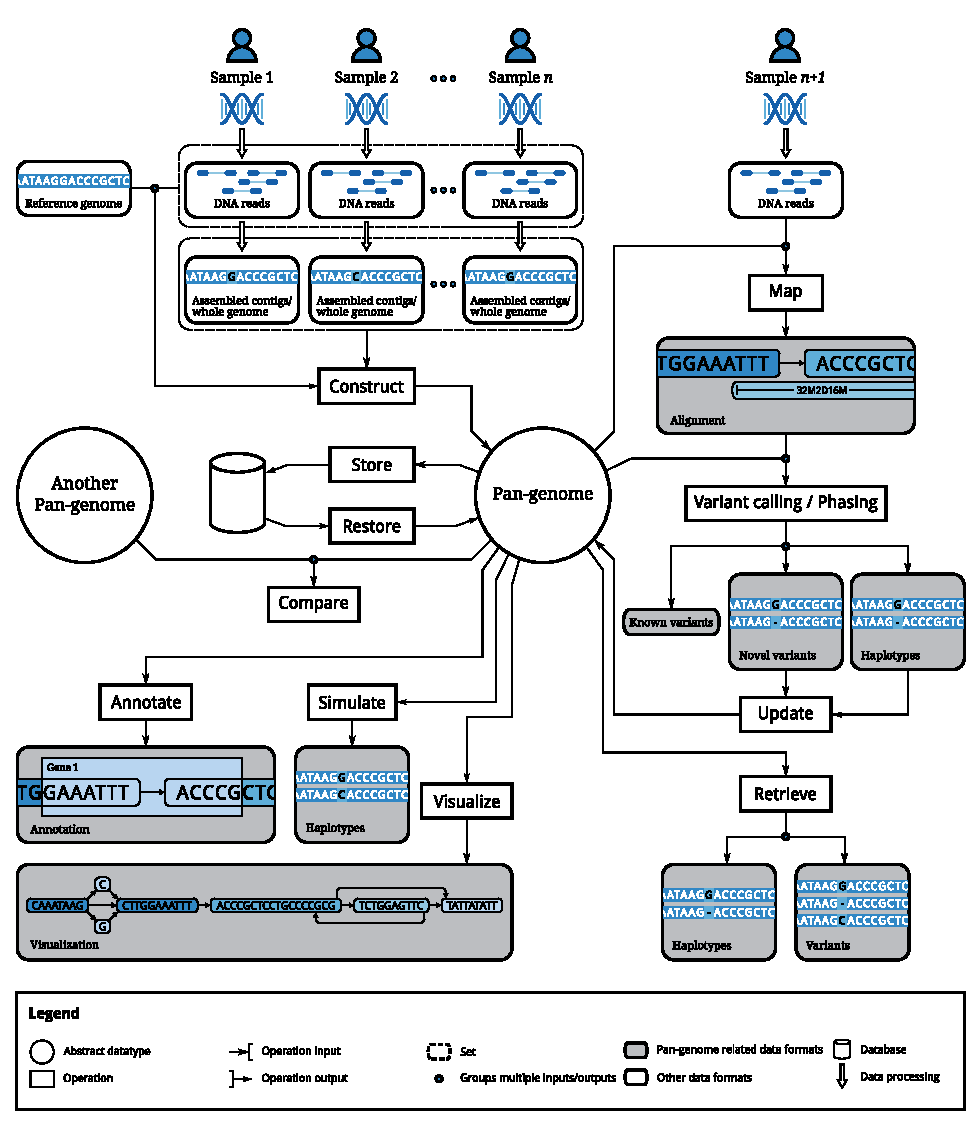
\includegraphics[width=1.0\textwidth]{Chapter1/Figs/cpang_fig2.pdf}
  \caption[Computational pangenomics]{
    An overview of techniques required to support pangenome-based resequencing.
    In {\tt vg}, we have implemented virtually all the presented components and algorithms.
    Reprinted from \cite{computational2016computational}.
    } 
\label{fig:pangenomic_processes}.
\end{figure}


% various approaches to encoding the pangenome

% think through, with references, the various ways we can resolve reference bias
% extended
\subsection{On pangenomic models}

\label{sec:on_pangenomic_models}

My own work builds on a particular model for encoding a pangenome.
Here, I will briefly describe alternative models and justify the use of the graphical one that I present, while the remainder of the chapter will provide background on more-closely related graphical approaches more closely related to my work.

Traditional techniques from microbial pangenomics have focused on cataloging the distribution of ORFs across bacterial species \cite{page2015roary}.
In this sense the pangenome is not so much a sequence-based object, but a matrix encoding the presence or absence of genes across the species of a given clade.

If we want to use pangenomic principles to resolve issues with resequencing, then we must take the concept of pangenome more literally, and build a representation that losslessly encodes genomes together with a focus on their sequence content.
In this perspective, the classical bacterial pangenome becomes a derivative product that we can produce using analyses based on a sequence-oriented pangenomic reference.
I will mostly focus on sequence-based pangenomic models.
The main classes are described visually in figure \ref{fig:pangenomic_models}.

\begin{figure}[htbp!]
  \centering
  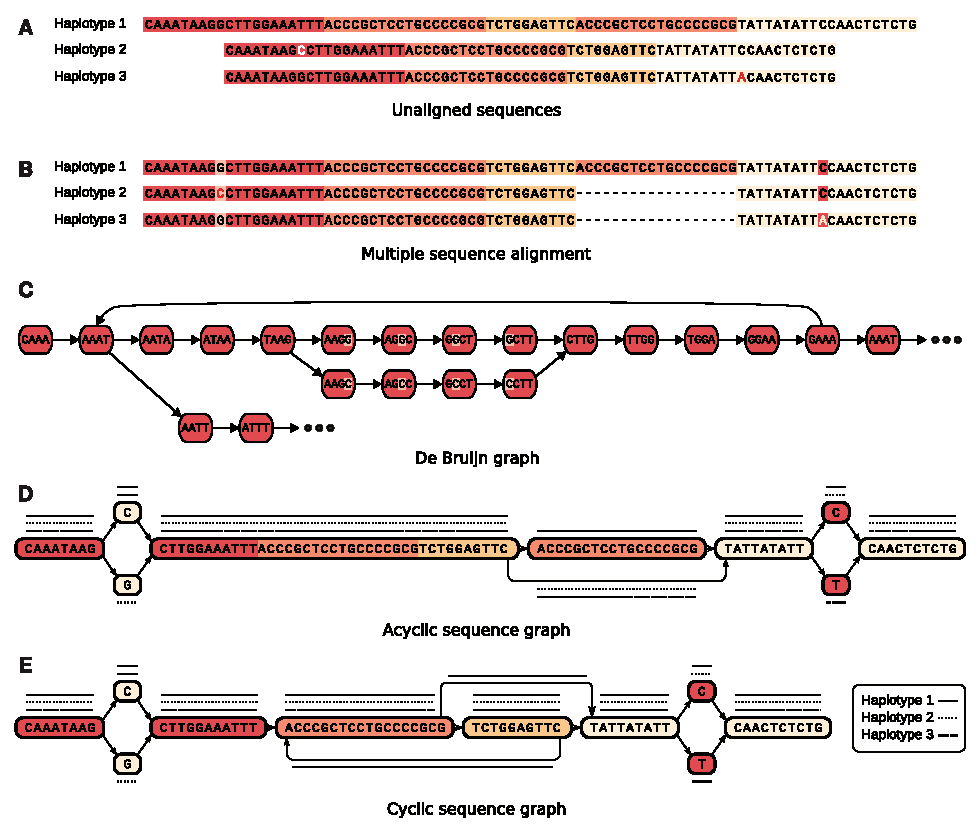
\includegraphics[width=1.0\textwidth]{Chapter1/Figs/cpang_fig3.pdf}
  \caption[Pangenomic models]{
    Various pangenomic models of a small collection of sequences.
    (A) shows an unfolded pangenome,
    (B) provides an MSA encoding the same sequences,
    (C) shows the DBG with $k=3$,
    (D) is an acyclic version of the pangenome, akin to the alignment in (B),
    and (E) represents a compressed alignment graph allowing cycles to represent copy number variants. 
    Reprinted from \cite{computational2016computational}.
    }
  \label{fig:pangenomic_models}.
\end{figure}

The simplest possible sequence-aware pangenome is just a set of whole genome sequences of many species or individuals, in which all sequence homologies and evolutionary relationships are implicit (figure \ref{fig:pangenomic_models}A).
The unfolded pangenome resolves reference bias, and can be extended with new data by simply including new genome sequences.
This model does not benefit from compression related to shared sequences in the pangenome, as adding a new genome always adds all the sequence in that genome to our system.
Without additional information about homologies, an unfolded pangenome cannot represent new sequences in terms of recombinants between known sequences.

An MSA (figure \ref{fig:pangenomic_models}B) provides a matrix describing the relationships between the sequences as well as the sequences themselves.
We must introduce a concept of a gap character to pad the matrix.
The MSA is a linear object, and cannot represent structural variation compactly.
An MSA has an equivalent representation as a sequence DAG, as in figure \ref{fig:pangenomic_models}D.

Assembly graphs, in particular DBGs (figure \ref{fig:pangenomic_models}C), provide a simple decomposition of collections of genomes.
However, a strict DBG without any labeling loses the mapping back to the original genomes.
Sequence graphs, as in figure \ref{fig:pangenomic_models}E, when annotated with the full set of input paths, provide a lossless representation of the input genomes.
If they are also bidirectional like DBGs (not shown in figure \ref{fig:pangenomic_models}E) then they can directly represent copy number variations and inversions.

\subsection{The variation graph}
\label{sec:the_variation_graph}

In this thesis I employ a reference system that encodes genomes and the base-level relationships between them.
This model can be understood as a kind of all-versus-all alignment between the sequences in the pangenome.
If the data model is to allow recombination between known sequences (a key contributor to genomic diversity) and tandem repeat copy number variation (which occurs readily in genomes), then it can be represented as a regular language encoded in a graphical model like a nondeterministic finite automaton (NFA).

We can adjust the regular language model slightly so that it has properties similar to those of DNA.
NFAs are represented graphically with states (in our case, pangenomic coordinates) as nodes connected by edges labeled by characters (e.g. DNA bases) in the alphabet of strings that the language recognizes.
In DNA the atomic element is the DNA base, which is represented as a character.
Graphical models with nodes (or edges) labeled by sequences and edges (or nodes) representing allowed transitions between them are a straightforward generalization of the linear string.
Compression can be achieved by allowing the labels on the nodes to have more than a single character on them.
Because DNA is double-stranded, any such a language implies a reverse complement language which recognizes the reverse complement of any sequence in the first.
Formalizing this by allowing edges to transition between different strands of the graph allows the model to directly represent sequence inversions.

If we combine these adjustments, we arrive at a kind of regular language model that resembles DNA and allows the representation of collections of related sequences by allowing us to represent homologous sequences and all kinds of natural polymorphism between them.
This structure is often referred to as a \emph{bidirectional DNA sequence graph}, indicating that the graph is sequence-centric, directed, stranded, and allows transitions between strands.
\emph{Sequence graph}, then implies a simpler concept in which the graph is meant to model sequences but only one strand is considered.
Assembly and multiple sequence alignment methods have employed sequence graphs of both types since the earliest computational analyses of biosequences, and it is sensible that we might employ them to represent collections of genomes.

The conceptual basis of the work I present here is the extension of the bidirectional DNA sequence graph with \emph{paths} that may be used to describe sequences as walks through the graph.
In this way, the panel of reference genomes or sequences used to construct the graph may be related to the graph itself, and the relationships between them made evident in the structure of the graph.
Existing knowledge expressed with respect to known sequences may thus be projected into the graphical pangenome model.
Similarly, entities within the graph may be \DIFdelbegin \DIFdel{``surjected'' }\DIFdelend \DIFaddbegin \DIFadd{projected }\DIFaddend out into the space of a given path \DIFaddbegin \DIFadd{(as described in section \ref{sec:surjection})}\DIFaddend .
These properties ensure that the pangenome fully encompasses existing reference technologies.
In addition, maintaining the sequences in the space of the graph makes the graph lossless, in that it fully represents the input sequences without additional information.
Perhaps most importantly, this feature resolves the exponential decay in mutual information which limits the applicability of Markovian models like the sequence graph to modeling natural sequences \cite{lin2017critical}.
I term this combination of a bidirectional sequence graph and paths a \emph{variation graph}, as it represents sequences and the variation between them.
In chapter 2 I will formalize the variation graph model and important auxiliary data structures that enable its modification and use in resequencing.

\section{Graphical techniques in sequence analysis}
\DIFaddbegin \label{sec:graphical_techinques}
\DIFaddend 

Many genome analysis algorithms employ sequence graphs.
I introduced the alignment algorithms described in \ref{sec:sequence_alignment} in terms of a matrix, but they may also be described as algorithms on graphs, although the nodes in these graphs correspond to matrix cells and thus alignment states rather than characters or sequences.
Similarly, hidden Markov models (HMMs) have a long history of use in bioinformatics \cite{durbin1998biological}, and these models bear similarities to the bidirectional sequence graph model.
Here, I will focus on those methods that are most closely related to variation graphs, and upon which my work draws most heavily.
These include techniques for generating and encoding multiple sequence alignments, genome assembly graphs, RNA splicing graphs, and the related gene model graphs used in RNA sequence analysis, and the sequence DAG implied by the VCF format.

\subsection{(Multiple) sequence alignment}
\label{sec:MSA}

Optimal multiple sequence alignment generalizes the problem of pairwise sequence alignment from a 2D matrix to an $N$-dimensional lattice, where the optimal mutual alignment of $N$ sequences of average length $L$ can be determined in $O(L^{N})$ time \cite{carrillo1988multiple}.
In the early days of sequencing, when only a handful of sequences might be considered in one analysis, such costs were almost acceptable, even if they limited the number of sequences in the MSA to only 3.
By pruning regions of the lattice in which no optimal alignments could occur, the authors of the tool ``MSA'' increased the number of sequences which could be optimally aligned into an MSA to 6 \cite{lipman1989tool}.
In contrast to the optimal alignment approach, progressive multiple sequence aligners such as CLUSTAL build a guide tree based on alignment of all sequences to all others in $O(NL^{2})$ time, and then generate the MSA progressively using the guide tree in $O(L^{2}\log N)$ time, resulting in polynomial time algorithms capable of generating MSAs for hundreds of sequences using contemporary computers \cite{higgins1988clustal}.
In this form of progressive alignment, the MSA is built recursively from the leaves to the root of the guide tree, with each step combining pair of MSAs representing different branches of the tree using the best pairwise alignment between the sequences they contain.
The progressive approach is fundamentally greedy, and susceptible to errors that propagate along the guide tree, although such errors can be mitigated by structuring the alignment using biological priors \cite{thompson1994clustal}.
Further improvements to the quality of the MSA can be gained by guiding the progressive alignment with a limited kind of global information about the relationships of all the sequences, as in T-COFFEE \cite{notredame2000t}, but this popular method exhibits a worst-case computational complexity of $O(N^{3}L^{2})$.

The progressive alignment in MSA algorithms like CLUSTAL may be represented graphically.
In the late 1980s Eugene Myers and Webb Miller developed algorithms to optimally align sequences to sequence graphs, and sequence graphs (in the form of regular expressions) to each other in $O(MN)$ time (where $M$ and $N$ are the sequence length of the graphs) \cite{myers1989approximate,wu1995subquadratic}.
Unfortunately, to my knowledge were never implemented in publicly available software for sequence analysis\footnote{Myers was unable to provide related source code on request.}.
A recent implementation of sequence to graph alignment \cite{rautiainen2018bit} transforms a sequence graph into an alignable graph which is acyclic and partially ordered, on which a bit-parallel alignment algorithm is applied to achieve high performance when aligning long noisy reads to arbitrary sequence graphs.
This work is related to that of Wu, Manber and Myers \cite{wu1995subquadratic}, wherein the authors provide an algorithm for the alignment of pairs of regular expressions using a transformation of the regexes to NFAs and bit-parallel resolution of the final alignment.
Later in chapter 2 I will present and evaluate a similar approach to align reads to arbitrary bidirectional sequence graphs through transformation of the graph into an ordered graph against which accelerated sequence to graph alignment may be run.

Christopher Lee later provided the first implementation of an MSA algorithm based on sequence to graph alignment \cite{lee2002POA}.
Apparently unaware of the work of Myers and Miller, he instead built on the concept of ``consistent equivalence relations'' that DIALIGN used to represent the MSA \cite{morgenstern1996multiple}.
Where DIALIGN's authors appear to consider the MSA in the space of the $N$-dimensional lattice, Lee encoded the equivalence relations in a partial order graph, which is often referred to as a directed acyclic graph (DAG).
In this DAG, characters label nodes and edges label observed linkages between them in sequences embedded in the MSA.
Lee demonstrated that a straightforward generalization of the recurrence relations used in Smith-Waterman-Gotoh would allow the alignment of sequences of length $N$ to the DAG of sequence length $M$ in approximately $O(MN)$ time.
To determine the score at a given position, partial order alignment (POA) considers matches and deletions relative to all the characters that immediately preceded the current one in the partial order.
Later, POA was extended to allow the direct alignment of pairs of MSAs using partial order to partial order alignment (PO-POA) \cite{grasso2004combining}.
Like CLUSTAL-W and other progressive methods, POA would build its MSA using pairwise alignments across a guide tree.
But, rather than aligning the last pair of sequences, PO-POA alignment would be used to align the MSAs from each branch together.
This resolved problems with order dependence, yielding MSAs with nearly the same accuracy\footnote{Here goodness is quantified using a sum of pairs score (SPS) metric representing the goodness of the alignment.} as T-COFFEE across a range of problems.
As PO-POA proceeds over a neighbor joining guide tree, it requires $N \log{N}$ alignment steps.
Given low sequence divergence, the cost of each step will approximate $L^2$.
The algorithm thus has a lower bound of approximately $O(L^{2}N\log{N})$, which the authors confirmed with experiments demonstrating subquadratic scaling in the number of input sequences.

Despite its use of an algorithm that scales cubically with the number of input sequences, T-COFFEE's higher accuracy has resulted in it receiving ten times the citations of POA.
The low rate of use meant that the POA concept was ``rediscovered'' by participants in the 1000GP who needed a computationally inexpensive method to align sequences to VCF-based pangenomes\DIFdelbegin \footnote{\DIFdel{Sequence to graph DAG alignment was one of Deniz Kural's main PhD projects. I worked with him in Gabor Marth's laboratory, and we applied his implementation of POA to generate accurate genotype likelihoods for indels and complex variation in the final phase of the 1000GP. We learned of the prior work later, when a reviewer pointed out that the algorithm was roughly equivalent to POA.}}%DIFAUXCMD
\addtocounter{footnote}{-1}%DIFAUXCMD
\DIFdel{.}\DIFdelend \DIFaddbegin \DIFadd{.}\footnote{\DIFadd{Sequence to graph DAG alignment was one of Deniz Kural's main PhD projects. I worked with him in Gabor Marth's laboratory, and we applied his implementation of POA to generate accurate genotype likelihoods for indels and complex variation in the final phase of the 1000GP. We learned of the prior work later, when a reviewer pointed out that the algorithm was roughly equivalent to POA.}}
\DIFaddend 

Lee's POA model provides a simple pattern for thinking about pangenomes.
However, POA MSAs are linear objects which cannot capture many natural kinds of genetic variation such as repeats or rearrangements without duplication of the rearranged sequences.
Several methods have extended the MSA concept to unordered graphs, including the Threaded Blockset Aligner (TBA) \cite{blanchette2004aligning}, which models the MSA graph as a set of partially ordered MSAs linked by unordered larger scale connections, and the A-Bruijn Aligner (ABA), which models the MSA using a de Bruijn graph and represents a solution to problems in MSA using techniques that later become important to short read assembly \cite{raphael2004novel}.
Variation graphs generalize these models without the limitations of order (as in POA and TBA) or $k$-mer based graph structures (as in ABA).

\DIFaddbegin \DIFadd{The POA model also inspired the development of a graphical model that supports the comparison of various editions or versions of the same text in the field of textual criticism, the }\emph{\DIFadd{variant}} \DIFadd{graph \mbox{%DIFAUXCMD
\cite{schmidt2009data,haentjens2014computer}}\hspace{0pt}%DIFAUXCMD
.
The variant graph can be understood as a POA DAG built from a collection of texts, whose nodes are labeled by the input texts that traverse them.
}\emph{\DIFadd{Variant}} \DIFadd{graphs are very similar to the }\emph{\DIFadd{variation}} \DIFadd{graphs that I present in this thesis, but while variant graphs are specialized for linear written texts, variation graphs aim to model DNA and genomic variation.
Although they have similar structure, these two models are in fact an unusual instance of interdisciplinary convergent naming.}\footnote{\DIFadd{I developed the term ``variation graph'' without knowledge of this prior work. I first become aware of it in the week before the initial submission of this thesis, when Daniel Bruder brought textual variant graphs to my attention. In practice, some researchers use both terms to refer to the model I present in this thesis.}}
\DIFadd{Variant graphs are used mostly to reduce the effort required to collate and manually review different versions of texts.
Recent work has focused on their visualization, resulting in techniques that are very similar to those developed for variation graphs which I present later in this thesis \mbox{%DIFAUXCMD
\cite{janicke2015traviz}}\hspace{0pt}%DIFAUXCMD
.
}


\DIFaddend \subsection{Assembly graphs}

The problem of assembling large genomes is not dissimilar from that of multiple sequence alignment.
MSA algorithms tend to be applied to the alignment of a single coherent genomic locus.
Their input sequences might be expected to have approximately the same length, and maintain synteny between them.
In contrast, whole genome shotgun assembly methods cannot rely on such assumptions, as reads of a large genome rarely overlap, and both strands of DNA will be sampled, yielding ambiguity about relative orientation.
Thus, the graphical models used in assembly must maintain bidirectional structure.
OLC assembly methods in some sense began their evolution with the set of compromises that MSA algorithms ended theirs, with thrifty heuristic methods being used to establish the overlaps between all pairs of sequence reads from a given genome, and the resulting overlap set subsequently represented graphically.
Earlier in section \ref{sec:genome_assembly} I gave a historical outline of the development of these methods in response to changes in available sequencing technology.
Here, I provide deeper technical detail to describe these methods and illustrate their relationship to the variation graph model.

\subsubsection{Overlap graphs}
\label{sec:overlap_graphs}

One interesting feature of overlap-based assembly graphs is that their efficient construction tends to yield a representation in which sequences attached to nodes partially overlap with the nodes in their neighborhood in the graph\footnote{In many formulations, sequences in the overlap graph are attached to edges rather than nodes. This model is equivalent to one in which sequences are attached to nodes, which I will use here for consistency. The same convention is used in {\tt vg}'s data model and in the GFA interchange format that it reads and writes.}.
This follows from the fact that the graph induction algorithms use a kind of pairwise alignment, retaining relationships between sequences in a pairwise rather than compacted N-wise form.
In the case of DBGs and the FM-index based string graph assemblers, an iterative overlap-wise sequence comparison where unitigs (unbranching sequences in the graph) are inferred from the compressed sequence graph yields overlap graph.
Given a node-labeled sequence graph, it is common to think of the edges as representing the overlaps between the nodes they connect.
This represents an incomplete compression of the relational information in the graph, but this is typically not important to the use of these methods.
They are judged by the quality of the set of contiguous sequences (contigs) they output rather than their raw assembly graph.
These methods will traverse linear portions of the graph to generate contigs, after pruning or ignoring edges, which the uncompressed overlap representation does not inhibit.

Due to its duplicated representation of sequences within overlaps, the overlap graph model is more complex to use as a reference system (in which positions should be unique) than a ``bluntified'' representation in which the overlaps are non-ambiguously reduced into the nodes in the graph and its linkage topology.
In their most general form, overlaps are themselves alignments, and have a natural encoding in graph form (section \ref{sec:MSA}).
However, assembly data models often encode alignments using several dissimilar data structures, a fact which is reflected in the complexity and redundancy of the GFA version 2 specification\footnote{\url{https://github.com/GFA-spec/GFA-spec/blob/master/GFA2.md}}.
In general this overlap representation makes it difficult to work directly with such graphs using the algorithms we will introduce, and they must be reduced into a ``blunt-ended'' bidirectional graph.

% mention miniasm and friends, bit of grounding in the present

It is also possible to directly induce a bidirectional string graph from a set of pairwise alignments, sidestepping the overlap issue.
In section \ref{sec:from_pairwise_alignments} I will present my design and implementation of an external memory algorithm that transforms sets of pairwise alignments into a variation graph using a transitive closure of the equivalencies implied by the alignments.

\subsubsection{De Bruijn graphs}
\label{sec:de_bruijn_graphs}

De Bruijn graphs \cite{de1946combinatorial} are graphs in which a set of $k$-mers are taken as the nodes of the graph, and edges are added for each pair of $k$-mers $k_1 \rightarrow k_2$ in which the last $k-1$ bases of $k_1$ are the same as the first $k-1$ bases of $k_2$.
As discussed previously in section \ref{sec:genome_assembly}, this model simplifies the overlap graph structure, allowing efficient calculation and representation of the graph.
For instance, $k$-mer lengths may be chosen so that they fit inside a machine word, allowing bitwise operations and integer math rather than string comparison to be used to infer the graph structure directly implied by the $k$-mers themselves.

In second generation sequencing, where per-base error rates are low and read lengths are short, little information is lost by breaking the read set into $k$-mers of 1/3 or 1/5th the length of the original reads, and so the de Bruijn graph model has been readily applied to cheap short read sequence data since its introduction to genomics in the mid 1990s and early 2000s \cite{idury1995new,pevzner2001eulerian}.
Velvet \cite{zerbino2008velvet}, which used a straightforward but memory-costly hash table strategy to encode the DBG.
Zamin Iqbal then extended the DBG model to support various kinds of pangenomic analysis by labeling each $k$-mer with ``colors'' representing read counts from different samples \cite{iqbal2012novo}.
The colored DBG (cDBG) model has seen application in RNA-seq transcript quantification, where the model is used as a reference basis for the relation of known transcripts to pseudoalignments of reads to the cDBG \cite{bray2016near}.
Later versions of the Cortex assembler have extended this to fully encode long reads or contigs relative to the DBG \cite{turner2018integrating}.
Similarly, improvements in performance have been yielded by linking read pairs in the DBG model \cite{bankevich2012spades}.

The simplicity of the DBG has made it possible to develop very memory-efficient data models to support its use in assembly.
The DBG can be effectively encoded in the FM-index of a read set \cite{bowe2012succinct}, and this \emph{succinct} DBG model underpins the most-scalable assembly methods currently available \cite{li2015megahit}.
Other techniques, such as bloom filter encodings and minimizer partitioning schemes are also used to provide time and space efficiency to DBG methods \cite{chikhi2013space, chikhi2016compacting}.

In the compacted DBG generalization non-furcating regions of the graph are merged into a single node with label length $>k$.
The compacted DBG is now often a typical output for DBG assemblers \cite{chikhi2016compacting,minkin2016twopaco}.
The compressed nodes and their overlaps with their neighbors comprise a set of unitigs that, together with their neighbor relations, are often taken as the most-raw kind of assembly output.
DBG assemblers like SPAdes and Minia3 infer longer contigs by filtering and further contracting the unitig graph \cite{bankevich2012spades}.

As with any overlap graph, DBGs must be made into blunt-ended sequence graphs before they can be utilized by variation graph based algorithms.
The basic method for doing so is simpler than for generic overlap graphs, as overlaps in DBGs are exact string matches.
In my work I have found this an important feature, as in addition to being generated by efficient methods, it ensures that DBGs are universally convertible into variation graphs.

\subsubsection{String graphs}
\label{sec:string_graphs}

The string graph is a formalism that describes the full information represented by a shotgun sequencing experiment and an all-against-all alignment between its reads \cite{myers1995toward,myers2005fragment}.
Myers argued that the then-current paradigm of assembly, which attempted to generate the shortest common superstring (SCS) incorporating all the $N$ input sequence reads, failed to reconstruct the genome correctly in the context of repeats in the genome that are longer than the average read length $L$.
He then posited the ``chunk graph'' (later, string graph) as a graphical model of the overlap set, showing that the correct consensus sequence would by definition exist as a walk through the graph, and that constraining the collapse using coverage information would improve reconstruction of the genome read in the shotgun sequencing experiment.
In this graph nodes (or edges) represent sequence reads and directed edges (or nodes) represented observed $\epsilon$-approximate overlaps between them.
Repeat units in the genome that are longer than $L$ will collapse in this graph, provided errors in the reads can be corrected so such repeats become fully identical.

This idea was introduced at the same time as de Bruijn graphs, with Myers' work on string graphs and the first description of a genome assembly algorithm using de Bruijn graphs both presented at the same workshop in 1995 \cite{myers1995toward,idury1995new}.
Myers' 2005 formalization of the string graph \cite{myers2005fragment} responds particularly to de Bruijn models, and he points out that generating $k$-mers from the reads as the basis for the graph means that the resulting graph is not ``read coherent'', or in other words does not accurately represent the information in the read set.
Subsequent work has shown that the boundaries between the two models are not so well-defined.
As a specialization of the overlap string graph, the de Bruijn model may be applied to certain complex subsets of a string graph, creating a kind of hybrid assembler where the $k$-mer model is used to resolve the most-difficult components, while the generic overlap model is used elsewhere \cite{huang2016integration}.
Similarly, the high cost of error and graphical complexity suffered by the string graph encourage the use of $k$-mer based read correction methods, which could be seen as filtering the reads using a DBG model.

String graphs are often described as ``lossless'' representations of the input read set and the alignments between them \cite{li2012exploring}.
Neither in practice, in Myers' formalizations, nor its implementations like the Celera assembler (CABOG) \cite{miller2008aggressive} is this strictly true.
In the model, overlaps are assumed to be $\epsilon-$correctable at approximately the raw sequencing error rate.
In practice, this filtering can result in a loss of input sequence from the string graph.
String graphs can consume very large amounts of memory when fully constructed without filtering from a read set \cite{li2016minimap,koren2017canu}.
Input filtering, mostly to reduce repeat content, is used to mitigate this issue.
If not aggressively corrected, repeats tend to generate ultra-dense graph regions that are known as ``hairballs'' which can increase the complexity of assembly by orders of magnitude.

To deal with repetitive sequences in the genome, one solution is to mask out repetitive $k$-mer, minimizer, or alignment seeds used in generating the overlap set, as in CABOG, FALCON, and miniasm \cite{miller2008aggressive,chin2016phased,li2016minimap}.
Recently, the authors of Canu showed that alternative probabilistic seed filtering based on the \emph{tf-idf} (term frequency, inverse document frequency) metric can retain information about repeats and support their separation rather than excision from the assembly string graph \cite{koren2017canu}.

String graph methods related to the Celera assembler, such as FALCON and Canu, implement error correction steps before overlap inference, as this reduces memory requirements during assembly.
Similarly, methods that generate assemblies via a string graph induction step from Illumina sequencing data (SGA, fermi, and fermikit) also apply an error correction processes before the generation of the string graph \cite{simpson2012efficient,simpson2014exploring,li2015fermikit}, which helps to reduce the graph complexity and improve contiguity of the resulting assembly.

Allelic diversity in either a string graph or de Bruijn graph will, if sufficiently separated from repeats and other allelic variants, result in a bubble, or graph component connected to the rest of the graph via single sources and sinks.
Like de Bruijn graphs, string graphs have been used to support variant calling, for instance finding heterozygotes represented as bubbles in the assembly graph \cite{li2012exploring}.
All methods that I am aware of will establish variants relative to a reference sequence threaded through the graph.
Also, thus far no method has specifically merged the two concepts of variant calling and graph based assembly finishing together, although assembly projects may use a variant caller to establish variants in their contigs \cite{jain2018nanopore,schmid2018pushing}.

With minimap and miniasm Heng Li took the approach of efficient all versus all alignment and overlap graph generation without prior read correction \cite{li2016minimap}.
With no multiple alignment step, this generates an assembly in which the error rate in the contigs approaches that of the input reads.
Tools like racon \cite{vaser2017fast} have been developed to subsequently generate a consensus, but these work on the level of individual contigs rather than an assembly graph.
Li \cite{li2016minimap} also proposed to mix and match different assembly components (for instance using DALIGNER \cite{myers2014efficient} rather than minimap for the overlap step, or swapping quiver for nanopolish for consensus generation) by establishing a set of standard data types including the pairwise alignment format (PAF) and the graphical fragment assembly (GFA).
These encode the results of the overlap step and a graphical model for the assembly at any state of its progression.
GFA is used in a wide number of methods, but as of August 2018 it appears that very few tools both read and write GFA\footnote{\url{https://github.com/GFA-spec/GFA-spec\#gfa-1}}, and much of the assembly improvement steps are implemented on contigs (encoded in FASTQ or FASTA format) rather than the string graph itself.

% it's an overlap graph yep

\subsubsection{RNA sequencing graphs}
\label{sec:rna_seq}

While many approaches to transcript analysis consider each particular gene transcript separately, a more compact representation would be as a \emph{splicing graph} in which all alternative splicing junctions are represented by edges connecting bases of the underlying reference sequence \cite{heber2002splicing,lee2002POA}.
Transcript assembly has attracted many of the same approaches as those used in genome inference, but their application must be adjusted to account for variation in read coverage of several orders of magnitude caused by large differences in expression of different genes \cite{martin2011next}, and in some cases they may not be suitable as the ideal of a transcript assembly is not a linear sequence assembly, but a splicing graph that models the combinatorial relationships in the transcriptome \cite{grabherr2011full}.
Standard assemblers, parameterized or modified to better support RNA transcript assembly have been applied to the problem since their development for genome assembly \cite{birol2009novo,robertson2010novo,schulz2012oases}.
But methods which are specifically design to meet the needs of the problem have arguably been more popular \cite{grabherr2011full,chang2015bridger}.

Direct use of the splicing graph concept is limited, with the most-popular workflow involving ``splice-aware'' alignment to a reference transcript model followed by quantification of expression versus the alignment and transcript model \cite{trapnell2012differential}.
More recently, probabilistic approaches have come into favor, and to support these assembly models have been applied to transcript quantification via pseudoalignment to a colored DBG annotated with reference transcripts \cite{bray2016near}.
In contrast, Daewan Kim's HISAT2 aligns RNA-seq reads to a whole genome splicing graph \cite{kim2015hisat,kim2017hisat2}, including SNP and indel variation directly in the whole genome index.

\subsubsection{Genome alignment graphs}
\label{sec:genome_alignment_graphs}
The graphs used in genome alignment algorithms are the nearest in content and structure to variation graphs, and it can be shown than a number them of nearly identical representational capacities \cite{kehr2014genome}.
The \emph{alignment graph}, first introduced in the context of multiple sequence alignment \cite{kececioglu1993maximum,rausch2008segment}, represents a collection of alignments in graphical form, supporting the induction of a sequence graph (or MSA when such a graph is partially ordered).
Vertices in the alignment graph $G_a = (V, E)$ represent characters in the input sequences $S$, and edges represent cases where characters in the input sequences have been aligned, with an additional relation $\prec$ on $V$ such that $v \prec w$ holds if and only if $v$ precedes $w$ in $S$.
As it contains both the sequences and their alignments, this graph may then be contracted to produce a compressed graph that represents both.
We can then contract $G_a$ into the base graph $G_s$, adding a node for each connected component in $G_a$ and labeling it with the corresponding character, while adding an edge for each pair of nodes $X$ and $Y$ which represent a pair of input characters in $G_a$ that satisfy $\prec$.
Each column of an MSA matrix or each base in a variation graph would correspond to a particular connected component in $G_a$.
It is worth noting that the equivalence is not exact unless we generalize the alignment graph to represent alignments in both the forward or reverse complement orientations, which has been explored in the A-Bruijn model \cite{raphael2004novel}.

The Enredo graph model $G_e = (V, E)$, used by Benedict Paten's Enredo/Pecan multiple genome aligner \cite{paten2008enredo}, generalizes the alignment graph model to be bidirectional by representing each genome segment in the graph with two nodes, a head and tail.
The graph maintains two kinds of edges, $E_s$ which represent genome segments and are equivalent to nodes in $G_s$, and $E_a$ which represent breakpoints of adjacencies between segments.
To obtain a graph like $G_s$ from the Enredo graph, the MSA resolver Pecan is applied to sets of homologous $E_s$ connecting the same head and tail nodes.

Paten further refined multiple genome alignment by the development of the Cactus graph $G_c = (V,E)$ \cite{paten2011cactus}.
To construct the Cactus graph, we build a precursor graph $G_c'$ by adding a node for each adjacency-connected component in the Enredo graph $G_e$ and adding edges between nodes for each segment $E_s$ whose head and tail lie in both adjacency components.
To obtain the Cactus graph, we collapse three-edge connected components in $G_c'$ into single nodes, yielding an Eulerian graph with a tree like structure.
The nodes in the Cactus graph can be shown to correspond to a tree of \emph{ultrabubbles} (graph components connected to the rest of the graph by one or two head and tail nodes) in the sequence graph from which it was constructed \cite{paten2018superbubbles}.
This forms the basis for the development of genotype models on top of arbitrary graphs.

Without additional labeling, these graph models are insufficient to fully reproduce their input, and although it may be implemented in corresponding software, existing models to do not clarify how this labeling is accomplished \cite{kehr2014genome}.
Variation graphs respond to this issue by making the path embedding of the sequences in the graph explicit in the model.

\subsection{Pangenomic alignment}

As the review presented in this chapter shows, the idea of using pangenomic models as a reference basis is not new, and interest in the topic extends back to the earliest explorations of the multiple sequence alignment problem.
But it was only in the last decade, as surveys of populations of genomes routinely produced sets of phased variant calls \cite{liti2009population,weigel20091001,cao2011whole,1000Gphase1,1000g2015} that the idea of scaling up alignment to enable the alignment of short reads to populations of genomes gained traction.
Numerous methods use some form of pangenome aware alignment.
These have helped me to understand the problem and guided my work to a significant degree.
Each has important limitations relative to more generic problems.
For instance, some operate on sequence DAGs, and cannot easily be generalized to work on arbitrary bidirectional sequence graphs.
Others implement a limited form of alignment that prevents their use for every kind of sequencing technology.
Virtually all use the pangenome only as an additional source of information during alignment, and do not use the pangenome as the reference system itself.

\subsubsection{Alignment to unfolded pangenomic references}

As discussed in section \ref{sec:on_pangenomic_models}, the simplest pangenomic model stores each genome sequence individually, without recording the implied homologies or relationships between the sequences.
Such a model grows linearly with the number of genomes included, and in this way it does not benefit from compression provided by sequence relationships and shared evolutionary histories.
Annotations can be provided for each genome and interlinked at a higher level of semantic relationships, as is done in major genome annotation catalogs like Ensembl genomes \cite{kersey2015ensembl}.
This expedient approach provides almost all the benefits of the kind of pangenomic models I present in this thesis, excepting that it cannot represent base-level sequence relationships within the semantic model without significant effort.
Whenever a researcher uses BLAST or BLAT to search a large database of sequence they are interrogating this ``unfolded'' pangenome.
This pattern could be thought of as the default in bioinformatics, and it is the starting place for many DNA-based analyses.

In terms of methods specifically designed to align large sequence read sets against an unfolded pangenome, few are currently under development.
Of note, the CHIC aligner provides an initial implementation of such an idea \cite{valenzuela2017chic}
This method is based on an indexing strategy which uses Lempel-Ziv (LZ77) \cite{ziv1977universal} parsing of the pangenome to generate a ``kernel'' sequence encoding the pangenome that may be indexed and used by a standard short read aligner (the authors use BOWTIE2).
By using this kernel, the seeding step is aware of alternative sequences embedded in the pangenome, but the local alignment step is ultimately run against a linear reference.
As this approach aligns directly to the unfolded pangenome it is not able to correctly estimate mapping quality, as the reference does not encode any model about the relationships between the genomes that comprise the pangenome and consequently we cannot determine when multiple alignments match to homologs in different genomes or paralagous copies dispersed across one or many genomes.
The linear growth in data scale can add algorithmic complexity when sequencing many genomes, and so it is understandable that experiments using the CHIC aligner only used up to 100 genomes at a time.
By relying on the linear reference to report alignments, CHIC gains the ability to hook into standard resequencing workflows, but it loses the ability to describe variation in sequence that is not contained in the reference.

%It is not clear yet if this model will be usable with practical inputs, and it is clear that it will not be able to encode other commonly-used graphical models for representing populations of genomes.
%Techniques from compressed data structures have been used to resequence short reads against the unfolded pangenome, as implemented in the CHIC aligner \cite{valenzuela2017chic}, but numerous problems have prevented the exploration of this modality.
%We can use this work to understand some limitations of this approach.


\subsubsection{Alignment to tiled pangenomic references}

A near-approximation of the unfolded model is one in which genomes are broken into small pieces in the construction of the model.
These blocks or tiles can then be formed into sequence DAG by the addition of edges showing linkages between successive blocks \cite{guthrie2015tiling}.
These models present as a specialized kind of sequence DAGs\footnote{Known implementations appear to be unable to directly represent inversions and copy number variants in their structures, instead encoding them as if they were indels.}, and can represent the whole set of sequences in a pangenome in a semi-compressed way using the same principles as in POA, DBG, or string graph models.
Each tile represents a known haplotype in a given window of the pangenome.
As new genomes are added to the structure, new tiles only need to be added where we observe a new sequence in a given window.

A tiled pangenome graph was employed by the pangenomic aligner, GenomeMapper \cite{schneeberger2009simultaneous}, which was produced in support of the \emph{Arabidopsis thaliana} 1001 Genomes Project (AT1001GP).
As arabidopsis frequently selfs, individuals may have extremely low levels of genomic diversity, which in turn simplifies the process of genome inference \cite{cao2011whole}.
At the same time, several percent of the reference genome is missing or highly divergent in various accessions (strains) \cite{clark2007common,zeller2008detecting}.
These conditions break standard short-read aligners developed for mapping Illumina sequencing data against low-diversity reference genomes.
GenomeMapper models the pangenome using 256 basepair tiles.
A $k$-mer index is used to seed local alignment of very short (<50bp) reads against the pangenome.
The authors report an extension of the Needleman-Wunsch alignment algorithm that allows alignment against the graph wherein the graph traversal is converted into a tree of alignments by duplicating the alignment process at each furcation.
This alignment algorithm is exponential in the average number of forks per sequence base, which may contribute to the observation that it runs hundreds of times slower than standard alignment methods on 100bp reads \cite{liu2016debga}.
GenomeMapper does not have a graph-specific alignment format, and instead reports alignments against the genome to which each is most similar, which the authors call ``reference free''.
So that the alignments may be used downstream in standard approaches, they may be projected against another chosen reference genome.

\subsubsection{Alignment to graphical assembly models}

In order to report their results relative to the reference, assembly methods require the ability to align the reference genome into the sequence graph they have generated \emph{de novo} \cite{iqbal2012novo,simpson2012efficient}, although this can be achieved through the alignment of the assembly graph's unitigs to the reference genome \cite{li2015fermikit}, which results in greater sensitivity to small variation but may also increase bias towards the reference genome.
Aligning external sequence to an assembly graph is equivalent to extending the assembly to include the sequence and recording the path through the assembly graph that represents it.

The deBruijn Graph Aligner (deBGA) inverts this approach by enabling the alignment of short reads to a reference DBG (RdBG) \cite{liu2016debga}.
An RdBG is a compacted DBG in which one or more reference genomes have been embedded, and the authors of deBGA enable alignment against it through a $k$-mer index that is used to drive a kind of MEM-based seed and extend alignment.
The alignment process itself attempts to link patterns of $k$-mer hits in unitigs in the graph into larger alignments, finally producing a local alignment by applying Smith-Waterman-Gotoh to the read and the particular reference genome region to which it aligns.
While deBGA uses a DBG to structure alignment, it can output a BAM file against the linear reference genome for use in variant calling or other analyses.
The authors claim that deBGA is fast and, thanks to its use of a DBG-based index, robust to alignment problems introduced by repeats.
However, it is not clear how the method develops mapping qualities, and due to its inability to represent evolutionary homology or equivalence between regions of genomes, this would appear to be is a significant limitation of the reference data structure they have chosen.

deBGA is the first published method specifically designed to align short reads against arbitrarily-structured graph genomes.
While deBGA was designed to work on collections of linear references, the authors note that it would also be possible to apply the indexing strategy to any sequence graph, as $k$-mer enumeration may be used to convert any sequence graph into a DBG\footnote{Jouni Sir\'{e}n and I had implemented an aligner based on a DBG transform of an arbitrary sequence graph at the time of deBGA's publication. The authors of deBGA were apparently as unaware of our work as we were of theirs.}
The authors do not evaluate its operation on generic DBGs, and instead compare it to linear reference based aligners on the same collections of genomes.

\subsubsection{Genotyping using a sequence DAG}
\label{sec:seq_dag_vcf}
Variant calls in the VCF format, when combined with the reference genome to which they refer, form a sequence DAG that encodes all the genomes from which the calls were derived as well as novel recombinations between them.
As this feature of variant calls was appreciated, it led to the development of several methods which first map reads globally to a linear reference and then realign them locally to a variation-aware reference.
This can be shown to reduce reference bias, but it can only do so in a localized sense as this form of graph resequencing cannot change the global placement of reads.

By the final phase of the 1000GP \cite{1000g2015} it was apparent that indels and complex variation were more difficult to genotype than SNPs.
Their significance was appreciated by 1000GP subprojects that examined the putative functional effects of such variants \cite{challis2015distribution}, which motivated efforts to develop a high-quality variant set including them for the final release.
The best-performing methods for generating the SNP genotype likelihoods (GLs) were only able to model biallelic SNPs \cite{snptools}, and additional methods would be applied to derive GLs for non-SNP, non-biallelic variant types.

While participating in the project, Deniz Kural and I extended (as glia\footnote{\url{https://github.com/ekg/glia}}) a POA algorithm he had developed to realign poorly-mapped reads (such as those with softclips, many mismatches, gaps, or unaligned fragments anchored by their pair mates) to a sequence DAG created from the reference and candidate alleles in the region.
By projecting the alignment back into the reference space, we were able to generate a BAM output from glia.
I implemented improvements to freebayes that allowed it to genotype alleles represented by observations in these alignments, as well as contamination estimates that were essential to high-quality GLs in low-coverage data.
This pipeline outperformed alternatives, and was ultimately used to generate GLs for all non-SNP variation in the project.

The indels were integrated into the phased scaffolds provided by the SNPs through two cycles of genotyping.
In the first, GLs generated by the method were given to MVNcall \cite{menelaou2012genotype}, a multalleleic, site-independent phasing algorithm that can phase genotypes at a given site onto a fixed background haplotype scaffold.
The posterior genotype and phasing quality estimates produced by MVNcall, along with a number of other metrics related to indel sequencing error such as sequence entropy and homopolymer context, were then used to establish a support vector machine (SVM) classification model which was trained using data from high-quality genomes and applied to the full set of alleles to remove likely errors.
The final set of alleles were fed back through the glia, freebayes, and MVNcall process to ultimately produce the set of indels in the 1000GP phase 3 release.

Hannes Eggertson's GraphTyper \cite{eggertsson2017graphtyper} implements a similar workflow to the genotype likelihood generation method applied to the 1000GP indels.
In the GraphTyper pipeline, Illumina reads are aligned against the reference genome using a standard short read aligner.
Those alignments with soft clips and apparent differences from the reference are matched to a sequence DAG built from the reference and VCF in a window around the read's candidate mapping location.
GraphTyper matches short $k$-mers between the read and the sequence DAG using a $k$-mer index of the reference structure and 1bp-overlapping $k$-mers from the read.
This does not produce an alignment \emph{per se}, but rather a list of variant traversals supported by each read.
This transformation provides sufficient information to genotype the variants in the graph.
The pipeline may update its reference system so that it includes both known variation from other studies and new variation discovered during analysis.
GraphTyper uses the graph reference system internally to improve algorithm performance, but results are projected into the linear reference and the graph has no other representation than VCF.
This prevents the representation of ``nested'' variation or non-SNP or indel SVs.
GraphTyper's efficient and accurate performance on exceptionally large resequencing problems supports the authors' design decisions and firmly asserts the utility of the graph realignment approach.

Sibbesen and colleagues generalize the genotyping problem to arbitrary variation graphs with BayesTyper \cite{sibbesen2018accurate}.
They adopt a kind of pseudoalignment model in which exact $k$-mer matches between a read set and the reference are used to establish support for paths across bubbles in the variation graph.
These can then be used to build probabilistic models of genotypes for any kind of variation represented in the graph, both small (SNPs and indels), including nested variation.

\subsubsection{Population reference graphs}

Pangenomic references need not be used as a coordinate system in the same manner as the linear reference genome.
Instead, they can be used as a prior to infer most-likely underlying haplotypes of a given individual.
Further refinement can be achieved by aligning the read set back to the inferred haplotypes.
This approach makes sense if alignment against the pangenome is extremely costly, but efficient haplotype inference patterns can be applied to the genome.

Population reference graphs (PRGs) \cite{dilthey2015improved} are POA-like graphs in which sequences aligned by MSA are collapsed in the case of identity above a given $k$-mer size, which embeds some information about local phasing into the graph.
First assembled from long sequences, the PRG is then augmented with local variation information, with SNPs and indels added to all paths at appropriate positions.
Dilthey and colleagues develop a genome inference model based on the comparison of the PRG to a DBG built from reads from a given individual.
By comparison between these two structures, weighted by $k$-mer frequency in the genome and PRG, they provide sufficient annotations to the PRG to run an HMM on the graph to infer the most-likely underlying pair of haplotypes.
Short read alignment can be used to map the full reads back to these haplotypes in an \emph{ad hoc} manner in order to find new small variation against them and fully resolve their sequences.
The authors demonstrate that this method can be applied to the human MHC, where high sequence diversity frustrates methods optimized for typical regions of the human genome.

\subsubsection{Succinct pangenomic sequence indexes}
\DIFdelbegin %DIFDELCMD < 

%DIFDELCMD < %%%
\DIFdelend \DIFaddbegin \label{sec:pangenomic_sequence_indexes}
\DIFaddend %Given a sequence DAG 
% write the DAG into the index provided a number of structural limitations
% problems with nesting (yes could be corrected) and cost of large alphabet WT based FM-index

Generalizations of the FM-index to support indexing of sequence DAGs, or equivalently regular languages, yielded a number of short read to sequence graph aligners.
Such methods enable pattern matching against pangenome graphs in much the same way as done by FM-index based short read aligners.

The Generalized Compressed Suffix Array (GCSA) \cite{siren2011indexing,siren2014indexing} enables pattern matching against arbitrary finite regular languages.
It indexes a reverse-deterministic automaton\footnote{Reverse determinization ensures that each prefix of this automaton can only have a single starting position.} that encodes the sequence DAG implied by a VCF and reference genome.
To enable path queries, it builds the BWT based on the sorted prefixes of the language encoded in the automaton, adding support structures that allow pattern search as in an FM-index.
Additional support bitvectors akin to those used to encode and index labeled trees \cite{ferragina2005structuring} allow the traversal of the sequence DAG during query matching.
Sir\'{e}n constructs the index using the prefix-doubling method used to construct sorted suffixes, wherein prefixes and their starts and ends may be extended from length $L$ to $2L$ through a sort and join operation.
Because it indexes a memoryless automaton and the construction requires the enumeration of all the prefixes of the automaton, GCSA suffers from exponential costs in index generation in the order of the number of possible recombinations represented in the sequence DAG.
Careful curation of the pangenome allows the construction of the GCSA for the entire human genome in the memory of an available computer (1TB), provided the construction is broken into chromosomes and local complexity in the input sequence DAG is reduced.
Experiments with the GCSA used backtracking search as in BWA \cite{li2009fast} to directly align reads with differences from the indexed graph, but the method was not developed into a full-featured short read alignment method.

Alternative schemes make no fundamental change to the CSA/FM-index model, but rather embed information about particular kinds of pangenome graphs into the sequence that is indexed.
BWBBLE \cite{huang2013short} encodes SNPs by extending the reference alphabet to include ambiguity codes which match more than one DNA base.
To encode indels, it extends the reference by adding a sequence for each indel which includes the non-reference allele and the surrounding $2l$ bases of the reference.
The resulting index can support queries of up to length $l$.
A mapping between the positions in the extended reference and the original reference sequence space is used to project alignments from the extended reference to the base reference.
This approach is simple and allows for a linear-time indexing of the pangenome, but the added complexity of the extended reference and larger alphabet required to represent SNPs yield a query time that is 100-fold slower than the backtracking BWA method \cite{huang2013short}.

In gramtools \cite{maciuca2016natural}, a particular kind of sequence DAG is indexed in a large-alphabet CSA based on wavelet trees \cite{grossi2003high}.\footnote{Wavelet trees reduce the representation of a large alphabet of size $\Sigma$ into a tree of $O(\log{\Sigma})$ bitvectors that recursively partition the sequence space into each character.
These bitvectors may be compressed efficiently while maintaining accessibility, and by augmenting them with rank and select supports the entire structure can be used to determine the number of each class of character before a given position, or select the $i$th of a given character.
This allows for the implementation of $LF$ mapping on a CSA represented in a large alphabet.}
Maciuca and colleagues develop an encoding for a sequence DAG in which bubbles may not have any deeper internal structure, and any traversal across a bubble is required to contain sequence.
Effectively, bubbles contain a number of alternate alleles that may be represented as linear sequences, and conveniently, this kind of graph is exactly that which is used in VCF.
To build its vBWT index of the graph, gramtools linearizes the alt-bubble sequence DAG into an integer vector (the ``linear PRG'') in which DNA bases are represented normally while the structure of each bubble is encoded as a series of alternate alleles delimited by $i$, flanked by delimiters $i-1$.
Each bubble gets a unique even integer $i$, requiring the use of alphabets with millions of symbols.
A CSA-based FM-index is then built from the linear PRG.
The \DIFdelbegin \DIFdel{backwards search algorithm is augmented to consider the alternate alleles when it encounters an odd integer greater than 4 (the alphabet space allocated to DNA sequence encoding).
The }\DIFdelend use of a unique pair of integers for each bubble ensures that the alleles in the bubble will be sorted together in the CSA of the linear PRG.
\DIFdelbegin \DIFdel{The encoded bubble structure allows backward search to furcate across the alternative alleles , and a }\DIFdelend \DIFaddbegin \DIFadd{To support direct matching to the sequence DAG, the standard backwards search algorithm is augmented to consider the alternate alleles when it encounters an odd integer greater than 4 (the alphabet space allocated to DNA sequence encoding).
On encountering a bubble, the search algorithm adds }\DIFaddend new suffix array \DIFdelbegin \DIFdel{interval is added }\DIFdelend \DIFaddbegin \DIFadd{intervals for each alternate allele }\DIFaddend to a heap of intervals that are extended together at each step.
As this scheme results in an exponential increase in the number of suffix array intervals \DIFaddbegin \DIFadd{as a query traverses multiple variants}\DIFaddend , the input set of alleles must be structured in a way to reduce the density of bubbles.
In their experiments the authors set an allele frequency threshold and merge alleles within a certain window size into larger haplotype alleles\footnote{The algorithm used to convert the input VCF into the haplotype bubble form appears to be \DIFdelbegin \DIFdel{the same as in }\DIFdelend \DIFaddbegin \DIFadd{similar to }\DIFaddend vcfgeno2haplo in vcflib: \url{https://github.com/vcflib/vcflib/blob/master/src/vcfgeno2haplo.cpp}.}.
It is perhaps due to this exponential factor that gramtools' query performance is many times slower than BWBBLE and around 1000 times slower than bwa mem on a linear version of the same reference \cite{maciuca2016natural}.
In effect, the method trades exponentially expensive construction for exponentially expensive queries.
Gramtools does not implement any local alignment model, and to demonstrate the method's conceptual utility, the authors apply it to infer the most-likely linear genome for a given query set, to which the read set is ultimately mapped using a standard aligner.

HISAT2 implements variation-aware alignment against human genome scale graphs, including alignment to RNA splicing junctions \cite{kim2017hisat2}.
Its hierarchical GFM-index structure allows seeding alignments against sequence DAGs.
To find seeds globally, it uses an implementation of the generalized compressed suffix array (GCSA) \cite{siren2011indexing}.
It builds the global index including common short SNPs and indels.
Then a set of local GCSA indexes are used to allow fast search of the splice graph and determination of candidate splicing junctions even when supported by minimal evidence in the read.
HISAT2 is an important point of reference as a scalable and mature implementation of sequence to graph alignment, and is presently the only widely-used aligner based on the GCSA index.
Like other methods, HISAT2 writes BAM alignments resulting from the expression of alignments to the sequence graph against the linear reference genome.
Unlike the other pangenomic aligners, HISAT2 can achieve very high throughput, and is competitive with standard short read aligners even when considering splicing and small variants.

Sir\'{e}n's more recent work on this topic has produced GCSA2 \cite{siren2017indexing}.
This model removes the automaton reverse-determinization step, allowing the index to be built on top of any kind of graph.
GCSA2 indexes a DBG generated from a bidirectional sequence graph in which nodes retain both $k$-mer identity and their starting and ending positional context in the graph.
This positional information is used to drive the prefix doubling step required to build the BWT of the DBG.
The space requirements of GCSA are avoided by terminating the prefix doubling at a length appropriate to accommodate queries of interest, which in practice is limited to 256bp.
By computing the longest common prefix array (LCP) of its sorted suffixes, GCSA2 encodes the implied suffix tree, which supports MEM-based seed generation algorithms for efficient and sensitive alignment against variation graphs.

\subsubsection{Mapping to \emph{k}-mer based pangenome indexes}

A $k$-mer index is trivial to build from a graph: one just needs to be able to enumerate or sample $k$-long walks through the graph and link the graph position to the $k$-mer in an efficient hash table or other kind of index.
The size of the index can be reduced by sampling $k$-mers in some pattern.
This indexing strategy was used in an early version of {\tt vg}, which supported experiments by the GA4GH-DWG \cite{novak2017genome} oriented at understanding the utility of various graphs constructed for a set of loci where GRCh38 encoded alternative sequences.
This same indexing technique is used by a proprietary method developed by members of the GA4GH-DWG from Seven Bridges Genomics Inc. (SBG) \cite{rakocevic2018fast}.
The SBG graph aligner's (SBGA) input is constructed from higher-frequency variants found in various public variation resources.
It masks out regions of high allelic complexity and builds a reference-rooted edge-labeled sequence DAG to serve as an alignment target.
To enable graph mapping it builds an index of spaced $k$-mers by walking short segments of the graph.
The $k$-mers and their locations are used as seeds to establish mapping candidate loci.
A local alignment is obtained for each candidate, and the output is transformed into the reference space as BAM.

Curiously, to align the reads to the graph locally SBG's aligner does not use a method like POA, and instead uses a kind of local backtracking exact matching against the tree of paths through the local graph which has exponential complexity with respect to the density of variation.
If the variant density and read error rates are kept low, this scheme allows SBGA to achieve extremely high read throughput, equivalent to that of bwa mem without any apparent loss in accuracy on the linear reference.
In this context the authors demonstrate their method can significantly (although slightly) improve sensitivity to known indels.
However, the method is not adaptable to other graph types or sequencing contexts, with reports from users indicating high increases in runtime with increased read error and variant density.
Due to the fact that SBGA is closed source and proprietary it is not possible to appreciate exactly why.

\section{Overview and objectives}

Resolving the genome of a sample \emph{de novo} requires sequencing and assembly.
Standard approaches to assembly are built on graphical models that allow for ambiguity, and out of this system they attempt to derive a set of contigs which represent the true haplotypes of the genome.
When we have already assembled a genome related to the one we wish to infer, we can describe our new sample in terms of a reference genome, with ambiguity and variation represented only in the alignments of the new sequences where they can be mapped to the reference genome.
This reduces the cost of sequencing, as we can infer much of the genome using lower sequencing coverage and shorter reads, but it also exposes resequencing based genome inference to reference bias, which is a distortion of inferred genomes towards the sequence of the reference genome.

I posit that by extending the reference genome to be a pangenome with a graphical representation, we can enable population aware resequencing that avoids reference bias to any particular linear reference.
The model I develop, the variation graph, extends the bidirectional sequence graph models used in assembly to support the labeling of paths through the graph, and allowing the representation and relation of linear reference systems within itself.

Variation graphs are related to a wide array of graphical models used in bioinformatics.
They have similarity with string graphs, multiple sequence alignments, and whole genome alignment graphs.
This indicates that they could serve as a unifying basis for many domains of sequence analysis which have traditionally been separated by methodological differences, such as assembly and variant calling.

Recently, several methods have been published which provide variation-aware alignment or genotyping based on sequence DAGs built from population resequencing.
These methods demonstrate the difficulty of the problem of generalizing resequencing to graphical reference systems at the multi-gigabase scale of vertebrate genomes.
In virtually all cases, they use a graph reference model internally, but express their results in terms of a linear reference genome, producing BAM alignments or genotyping results in VCF format.
None implement a generic strategy to work with a graphical model equivalent to the variation graph.
The method I develop, {\tt vg}, is not the first pangenomic aligner, but it is the first that models its results in terms of the pangenome itself, enabling full resequencing analyses to be completed within the graphical model.

In the following chapters I will precisely define the variation graph and associated data models that allow representing all kinds of resequencing data types in the context of a variation graph.
Then I will describe the algorithms implemented in {\tt vg} that enable the use of variation graphs as a basis for genome analysis, including their construction from many data sources, serialization and visualization.
I will present indexing methods that support the queries needed to enable resequencing, and I will provide algorithms that implement efficient read alignment to large scale graphs.
Finally, I will cover applications of the method I developed.
I will show that {\tt vg} is applicable to a wide range of genomic inference problems, with a particular focus on the quality of alignment of both short and long sequence reads against variation graphs constructed from all kinds of sources.

Throughout this work I use the first person singular \emph{``I''} to refer to work that I completed alone, while the plural \emph{``we''} where presenting work completed in collaboration with others.
Wherever possible, I clarify the nature of the collaboration and identify my collaborators.
